\documentclass[11pt]{report}

% ---------- Basic setup ----------
\usepackage[utf8]{inputenc}
\usepackage[T1]{fontenc}
\usepackage[english]{babel}

\usepackage{amsmath,amssymb}
\usepackage{physics}
\usepackage{graphicx}
\usepackage{mathptmx}          % Times-like font
\usepackage{fontawesome5}
\usepackage{xcolor}
\usepackage{geometry}
\usepackage{titlesec}
\usepackage{setspace}
\usepackage{fancyhdr}
\usepackage[most]{tcolorbox}

\geometry{a4paper, margin=2.0cm}
\setlength{\parskip}{0.7em}
\setlength{\parindent}{0pt}
\onehalfspacing

% ---------- Colors ----------
\definecolor{MLTeal}{HTML}{00897B}     % main teal
\definecolor{MLTealLight}{HTML}{E0F2F1}% light teal background
\definecolor{MLGray}{HTML}{455A64}     % dark gray for text accents


\definecolor{MLGray1}{HTML}{424242}          % dark gray for title text
\definecolor{MLGrayLight}{HTML}{E0E0E0}     % very light gray background
\definecolor{MLGrayFrame}{HTML}{9E9E9E}    

% ===== Coral Code Box =====
\definecolor{CoralPink}{HTML}{FF6F61}      % main coral color
\definecolor{CoralBack}{HTML}{FFE6E2}      % very light coral background




% ---------- Chapter style ----------
\titleformat{\chapter}[display]
  {\normalfont\huge\bfseries}
  {%
    \colorbox{MLTeal}{%
      \makebox[\textwidth][l]{\hspace{1em}\color{white}\thechapter}%
    }%
  }
  {1ex}
  {\Huge}

\titlespacing*{\chapter}{0pt}{4ex}{3ex}

% ---------- Section styles ----------
\titleformat{\section}
  {\Large\bfseries\color{MLTeal}}
  {\thesection}{0.8em}{}

\titleformat{\subsection}
  {\large\bfseries\color{MLGray}}
  {\thesubsection}{0.6em}{}

% ---------- Header / footer ----------
\pagestyle{fancy}
\fancyhf{}
\renewcommand{\headrulewidth}{0pt}
\fancyhead[L]{\textcolor{MLGray}{Notes for Understanding Machine Learning}}
\fancyhead[R]{\textcolor{MLTeal}{\thepage}}
\fancyfoot{}

% ---------- tcolorbox styles ----------
\tcbset{
  sharp corners,
  boxrule=0.8pt,
  colframe=MLTeal,
  colback=MLTealLight,
  left=1em,right=1em,top=0.7em,bottom=0.7em,
  enhanced,
}

\newtcolorbox{mlidea}[1][]{
  title={\faLightbulb[regular]~Key Idea},
  fonttitle=\bfseries,
  coltitle=MLGray,
  colback=MLTealLight,
  colframe=MLTeal,
  breakable,
  #1
}

\newtcolorbox{mlexample}[1][]{
  title={\faChartLine~Example},
  fonttitle=\bfseries,
  coltitle=MLGray,
  colback=white,
  colframe=MLTeal,
  breakable,
  #1
}

\newtcolorbox{mlnote}[1][]{
  title={\faStickyNote[regular]~Note},
  fonttitle=\bfseries,
  coltitle=MLGray,
  colback=MLTealLight,
  colframe=MLTeal,
  breakable,
  #1
}


\newtcolorbox{mlexample1}[1][]{
  title={\faBook~Example-Recap},
  fonttitle=\bfseries,
  coltitle=MLGray1,
  colback=MLGrayLight,
  colframe=MLGrayFrame,
  breakable,
  enhanced,
  sharp corners,
  boxrule=0.7pt,
  #1
}

\newtcolorbox{mlcode}[1][]{
  enhanced,
  colback=CoralBack,
  colframe=CoralPink,
  title={\faCode~Code Example},
  fonttitle=\bfseries\ttfamily,
  coltitle=white,
  boxed title style={
      colback=CoralPink,
      sharp corners,
      boxrule=0pt,
  },
  attach boxed title to top left={yshift=-2mm, xshift=4mm},
  breakable,
  top=6pt,
  bottom=6pt,
  left=6pt,
  right=6pt,
  #1
}


\usepackage{listings}
\usepackage{xcolor}

% -------- Python highlighting style (PyCharm-like) --------
\definecolor{pykeyword}{HTML}{005CC5}
\definecolor{pycomment}{HTML}{6A737D}
\definecolor{pystring}{HTML}{22863A}
\definecolor{pyfunc}{HTML}{6F42C1}
\definecolor{pybackground}{HTML}{F6F8FA}

\lstdefinestyle{pystyle}{
    backgroundcolor=\color{pybackground},
    commentstyle=\color{pycomment}\ttfamily,
    keywordstyle=\color{pykeyword}\bfseries,
    stringstyle=\color{pystring},
    identifierstyle=\color{black},
    basicstyle=\ttfamily\small,
    showstringspaces=false,
    tabsize=4,
    frame=single,
    rulecolor=\color{gray},
    frameround=tttt,
    breaklines=true,
    numbers=none,          % <---- removed line numbers
}



% ---------- Title ----------
\title{%
  \vspace{1cm}
  {\Huge\bfseries Notes for Understanding}\\[0.3cm]
  {\Huge\bfseries\color{MLTeal} Machine Learning}\\[0.3cm]
  {\large\itshape A personal learning textbook}
}
\author{{\Large\bfseries Ioanna Stamou}}
\date{\vspace{-0.5cm}}
\setcounter{tocdepth}{1}


\begin{document}

\maketitle

\tableofcontents
\clearpage

% ---------- Introduction ----------
\chapter*{Introduction}
\addcontentsline{toc}{chapter}{Introduction}

Imagine you have a robot friend.

You give the robot a task:

\medskip
\centerline{\emph{“Look at these examples, learn the pattern, and make predictions.”}}

\medskip
This is machine learning.

\begin{center}
\textbf{Machine learning = finding patterns in data.}
\end{center}

Example:

You give a model 1000 houses with their \emph{price}, \emph{size}, and \emph{number of rooms}.  
The model learns the relationship between these features and the price.  
Then, when you give it a \emph{new} house, it predicts the price.

That’s all.

\begin{mlidea}
Machine learning is not magic.
It is a systematic way to:
\begin{enumerate}
  \item collect data,
  \item find patterns,
  \item use those patterns to make predictions or decisions.
\end{enumerate}
\end{mlidea}

The rest of these notes are about:
\begin{itemize}
  \item the \textbf{statistics} you need to talk precisely about patterns,
  \item the \textbf{Python tools} you will use to work with data,
  \item the \textbf{machine learning algorithms} that actually learn from examples.
\end{itemize}

\clearpage

% =======================
\chapter{Statistics You Need for Machine Learning}

In this chapter we will develop the basic statistical ideas that appear everywhere in
machine learning: random variables, distributions, expectation, variance, covariance,
correlation, and a few key theorems that explain why learning from data can work.


\section{Types of Variables}

\subsection*{Numerical Variables}
Numerical variables take quantitative values.

\begin{itemize}
    \item \textbf{Continuous:} $x \in \mathbb{R}$  
          Examples: height, temperature, house price.
    \item \textbf{Discrete:} $x \in \mathbb{Z}$  
          Examples: number of rooms, number of customers.
\end{itemize}

\subsection*{Categorical Variables}
Categorical variables represent non-numerical classes.

\begin{itemize}
    \item \textbf{Nominal (unordered)}  
          Examples: color, country, type of food.
    \item \textbf{Ordinal (ordered)}  
          Examples: rating levels, education level.
\end{itemize}

\textbf{Important:} Machine learning models expect numerical inputs.  
Categorical variables must be encoded (one-hot, label encoding, etc.).

% ------------------------------------------------------

\section{Descriptive Statistics}

\subsection{Mean}
The mean (average) of $n$ observations is:
\[
\mu = \frac{1}{n} \sum_{i=1}^n x_i.
\]

\subsection{Median}
The median is the middle value of the sorted data.  
It is more robust to outliers than the mean.

\subsection{Variance}
Variance measures how far the values are spread from the mean:
\[
\mathrm{Var}(X) = \frac{1}{n}\sum_{i=1}^n (x_i - \mu)^2.
\]

\subsection{Standard Deviation}
Standard deviation is the square root of the variance:
\[
\sigma = \sqrt{\mathrm{Var}(X)}.
\]
It measures the typical deviation from the mean.

\subsection{Covariance}

Variance tells us how a single variable varies.  
Covariance tells us how \emph{two} variables vary \emph{together}.

\[
\mathrm{Cov}(X, Y) = \mathbb{E}\left[(X - \mu_X)(Y - \mu_Y)\right].
\]

Interpretation:

\begin{itemize}
    \item Positive covariance: when $X$ is above its mean, $Y$ tends to be above its mean.
    \item Negative covariance: when $X$ is above its mean, $Y$ tends to be below its mean.
    \item Zero covariance: no linear relationship.
\end{itemize}
% ------------------------------------------------------

\section{Correlation}

Correlation measures the strength of linear dependence between two variables.

\begin{itemize}
    \item Range: $[-1,1]$
    \item Indicates how two variables move together
\end{itemize}

\[
\rho_{XY} = \frac{\mathrm{Cov}(X,Y)}{\sigma_X \sigma_Y}.
\]

\begin{itemize}
    \item $+1$: perfect positive relationship  
    \item $0$: no linear relationship  
    \item $-1$: perfect negative relationship  
\end{itemize}

Machine learning uses correlation to select and weight relevant features.

% ------------------------------------------------------

\section{Probability Theory Basics}

Machine learning models predict probabilities.  
Even regression models assume probabilistic noise.

Key ideas:
\begin{itemize}
    \item \textbf{Joint probabilities}: describe combined events.
    \item \textbf{Conditional probabilities}: describe relationships.
    \item \textbf{Marginal probabilities}: describe overall tendencies.
\end{itemize}

This logic becomes the backbone of all ML algorithms.

% ------------------------------------------------------

\subsection{Joint Probability}
For events $A$ and $B$:
\[
P(A,B) = P(A \cap B).
\]

\subsection{Conditional Probability}
\[
P(A \mid B) = \frac{P(A,B)}{P(B)}.
\]

\subsection{Marginal Probability}

\textbf{Discrete:}
\[
P(A) = \sum_b P(A,b).
\]

\textbf{Continuous:}
\[
P(A) = \int P(A,b)\, db.
\]

Probability quantifies uncertainty.  
Conditional probability expresses relationships between events.

% ------------------------------------------------------

\section{Bayes' Theorem: Updating Beliefs from Data}

\subsection{Formula}

Bayes' theorem describes how we update our belief about an event $A$
after observing some evidence $B$:

\[
P(A \mid B) = \frac{P(B \mid A) \, P(A)}{P(B)}.
\]

\subsection*{What does this mean?}

Bayes' theorem tells us:

\begin{center}
\textbf{Posterior = Likelihood $\times$ Prior \; / \; Evidence}
\end{center}

More explicitly:
\begin{mlidea}
\[
P(A \mid B)
= 
\underbrace{P(B \mid A)}_{\text{How well $A$ explains the data}}
\;
\underbrace{P(A)}_{\text{What we believed before}}
\;
\Big/
\;
\underbrace{P(B)}_{\text{How expected the data is overall}}.
\]

\begin{itemize}
    \item $P(A)$ [ \textbf{prior}]  :
          What we believed before seeing any data.
    \item $P(B \mid A)$ [\textbf{likelihood}]  :
          How compatible the observed data $B$ is with our hypothesis $A$.
    \item $P(B)$ [\textbf{evidence}]  :
          The probability of seeing the data under all possible explanations.
    \item $P(A \mid B)$  [\textbf{posterior}]  :
          Our updated belief about $A$ after incorporating evidence $B$.
\end{itemize}
\end{mlidea}

\subsection*{Intuition}

Bayes' theorem answers the question:

\begin{center}
\emph{“Given what I just observed, how should I update what I believe?”}
\end{center}

It combines two ideas:

\begin{enumerate}
    \item \textbf{What we believed before} (the prior)
    \item \textbf{How surprising the data is under each hypothesis} (the likelihood)
\end{enumerate}

The evidence $P(B)$ ensures everything stays a valid probability distribution (sums to 1).

\subsection*{Why this matters in Machine Learning}

Bayes' theorem is the foundation of:
%\begin{itemize}
    Naive Bayes classifier, 
Bayesian Linear Regression, 
 Bayesian Neural Networks,
   All probabilistic and generative models. 
%\end{itemize}

It formalizes \textbf{learning from data}.  
We start with a belief (prior), then see data, and update our belief (posterior).


% ------------------------------------------------------


% ------------------------------------------------------

\section{Likelihood}

The concept of \textbf{likelihood} answers a very important question in
statistics and machine learning:

\begin{mlidea}
\begin{center}
\emph{“If this parameter $\theta$ were true, how well would it explain the data I observed?”}
\end{center}
\end{mlidea}

This is different from asking about the probability of future events.
Likelihood is specifically about evaluating how plausible a parameter
is, given the data we already have.

\subsection*{Definition}

For a dataset $x = (x_1, x_2, \dots, x_n)$ and a model with parameter $\theta$, the likelihood is defined as:

\[
L(\theta \mid x) = P(x \mid \theta)
\]

This expression should be read as:

\begin{itemize}
    \item[] \textbf{“Given $\theta$, what is the probability of observing the dataset $x$?”}
\end{itemize}

\subsection*{Interpretation}

\begin{itemize}
    \item $x = (x_1, x_2, \dots, x_n)$: the observed data.  
          These values are \textbf{fixed}. We already saw them.
    \item $\theta$: the parameter of the model.  
          This is \textbf{unknown} and is what we want to estimate.
    \item $P(x \mid \theta)$: the model’s prediction about how likely the data is, if $\theta$ were the true parameter.
\end{itemize}

\subsection*{Important Distinction: Probability vs. Likelihood}

\begin{itemize}
    \item \textbf{Probability:} $\theta$ is fixed, data is random.  
          (Used to predict future observations.)
    \item \textbf{Likelihood:} data is fixed, $\theta$ is variable.  
          (Used to evaluate or estimate parameters.)
\end{itemize}

This is a subtle but essential idea in statistical learning.

\subsection*{The Likelihood Function}
\begin{mlnote}
The likelihood function is simply the probability of the data, viewed as a function of the parameter:

\[
L(x ; \theta) = P(x \mid \theta)
\]

It tells us how much support the data gives to each possible value of $\theta$.

\begin{center}
\emph{“Better-fitting parameters give higher likelihood.”}
\end{center}

\textbf{Crucially:} likelihood is \emph{not} a probability distribution over $\theta$.  
It does \textbf{not} integrate to 1.  
It is just a scoring function that says which values of $\theta$ explain the data best.
\end{mlnote}

\subsection*{The i.i.d. Assumption}

In most machine learning models, the data points are assumed to be:

\begin{itemize}
    \item \textbf{independent:} knowing one datapoint tells nothing about another,
    \item \textbf{identically distributed:} all datapoints come from the same distribution.
\end{itemize}

Under this assumption:

\[
L(x \mid \theta) = \prod_{i=1}^n P(x_i \mid \theta)
\]

Why a product?

Because the joint probability of independent events equals the product of their individual probabilities.

This is a key simplification that makes likelihood computation possible for large datasets.

\subsection*{Summary}

\begin{itemize}
    \item Likelihood measures how well a model with parameter $\theta$ explains the observed data.
    \item It is the central tool for parameter estimation.
    \item Almost all ML algorithms rely on likelihood:
    \begin{itemize}
        \item Linear Regression  
        \item Logistic Regression  
        \item Neural Networks  
        \item Decision Trees and Random Forests (implicitly)  
        \item XGBoost  
    \end{itemize}
    \item Training a model often means:
    \[
    \text{maximize likelihood} \quad \text{or} \quad \text{minimize negative log-likelihood}.
    \]
\end{itemize}

In short, likelihood connects your model to your data.
It is the mathematical backbone of statistical learning.

% ------------------------------------------------------
\section{Probability Distributions: Shape of Data}

A probability distribution describes \textbf{how data behaves}.  
It tells us which values are likely, which are rare, and what kind of
uncertainty or randomness we should expect in the data.

Machine learning models often assume certain distributions because
they determine the model's behavior and how it handles noise.

% --------------------------------------------------------
\subsection{Discrete Distributions}

Discrete distributions describe random variables that take values
from a finite or countable set (e.g., 0, 1, 2, 3, ...).

% -------------------
\paragraph{Bernoulli Distribution}

A Bernoulli variable represents a single binary outcome:

\[
P(X = x) = p^x (1-p)^{1-x}, \qquad x \in \{0,1\}.
\]

Interpretation:

\begin{itemize}
    \item Models ``success or failure'' events.
    \item Examples: coin flip, email is spam/not spam, churning/not churning customer.
    \item Parameter $p$ is the probability of success.
\end{itemize}

% -------------------
\paragraph{Binomial Distribution}

The binomial distribution models the number of successes in $n$
independent Bernoulli trials:

\[
P(X = k) = \binom{n}{k} p^k (1-p)^{n-k}.
\]

Interpretation:

\begin{itemize}
    \item Repeating the same experiment $n$ times.
    \item Examples: number of heads in $n$ coin flips,
                    number of defective items in a batch.
    \item Gives the distribution of the \emph{count of successes}.
\end{itemize}

% -------------------
\paragraph{Poisson Distribution}

The Poisson distribution models the number of events occurring
in a fixed time or space interval:

\[
P(X = k) = \frac{\lambda^k e^{-\lambda}}{k!}.
\]

Interpretation:

\begin{itemize}
    \item Used for rare events happening unpredictably.
    \item Examples: number of incoming calls per minute,
                    number of website hits per second,
                    number of accidents per day.
    \item Parameter $\lambda$ is both the mean and the variance.
\end{itemize}

% --------------------------------------------------------
\subsection{Continuous Distributions}

Continuous distributions describe variables that take real-number values
(e.g., height, temperature, time).

% -------------------
\paragraph{Gaussian (Normal Distribution)}

\[
f(x) = \frac{1}{\sqrt{2\pi\sigma^{2}}}
\exp\left( -\frac{(x-\mu)^2}{2\sigma^{2}} \right)
\]

Interpretation:

\begin{itemize}
    \item The most important distribution in statistics.
    \item Data clusters around a mean $\mu$ with spread $\sigma$.
    \item Many ML models assume Gaussian noise.
    \item Examples: measurement error, natural variations, height.
\end{itemize}

% -------------------
\paragraph{Exponential Distribution}

\[
f(x) = \lambda e^{-\lambda x}
\]

Interpretation:

\begin{itemize}
    \item Models the time between independent random events.
    \item Examples: time until next earthquake, time until customer arrival.
    \item Memoryless property: past values do not change future probability.
\end{itemize}

% -------------------
\paragraph{Multivariate Gaussian}

\[
f(x) = \frac{1}{(2\pi)^{d/2} |\Sigma|^{1/2}}
\exp\left( -\frac{1}{2}(x - \mu)^T \Sigma^{-1}(x - \mu) \right)
\]

Interpretation:

\begin{itemize}
    \item A Gaussian distribution in multiple dimensions.
    \item $\mu$ is a mean vector, $\Sigma$ is a covariance matrix.
    \item Models correlated variables.
    \item Used heavily in:
    \begin{itemize}
        \item PCA (Principal Component Analysis)
        \item Gaussian Mixture Models (GMMs)
        \item Bayesian inference
    \end{itemize}
\end{itemize}

% --------------------------------------------------------
\subsection*{Why Distributions Matter in Machine Learning}

Different distributions encode different assumptions about uncertainty:

\begin{itemize}
    \item Bernoulli / Binomial → binary or count data  
    \item Gaussian → continuous data with natural noise  
    \item Poisson → rare event counts  
    \item Exponential → waiting times  
    \item Multivariate Gaussian → correlated continuous data  
\end{itemize}

Choosing an appropriate distribution helps us build models that
accurately reflect the data-generating process.

% ------------------------------------------------------
\section{Statistical Inference: Learning Parameters From Data}

Statistical inference is about using data to learn the best values for the
parameters of a model. In machine learning, almost every algorithm can be
understood as an inference method.

We focus on two fundamental ideas:
\begin{itemize}
    \item \textbf{Maximum Likelihood Estimation (MLE)}
    \item \textbf{Maximum A Posteriori Estimation (MAP)}
\end{itemize}

These appear throughout regression, classification, probabilistic models,
and even deep learning.

% ---------------------------------------------------------
\subsection{Maximum Likelihood Estimation (MLE)}

MLE answers a simple question:

\begin{mlidea}
\begin{center}
\emph{“Which parameter value makes the observed data the most likely?”}
\end{center}
\end{mlidea}

If $x = (x_1, \dots, x_n)$ is the observed data and $\theta$ is an unknown parameter,
the MLE estimate is \footnote{max $\rightarrow$ what is the highest value. argmax $\rightarrow$ where is the highest value}:

\[
\hat{\theta}_{\mathrm{MLE}} = \arg\max_{\theta} L(\theta \mid x)
\]

where

\[
L(\theta \mid x) = P(x \mid \theta)
\]

is the likelihood of the data under the parameter $\theta$.

\subsubsection*{Why do we take the log?}

Because products of probabilities become sums:

\[
\hat{\theta}_{\mathrm{MLE}}
= \arg\max_{\theta} \log L(\theta \mid x)
\]

This is numerically stable and makes optimization easier.

\subsubsection*{Intuition}

\begin{itemize}
    \item The data $x$ is considered fixed.
    \item The parameter $\theta$ varies.
    \item We choose the $\theta$ that best \emph{explains} the data.
\end{itemize}

This idea lies behind most ML algorithms: 
%
%\begin{itemize}
   Linear regression (least squares),
     Logistic regression, 
     Naive Bayes, 
     Neural networks (via cross-entropy).
%\end{itemize}

All of them optimize a likelihood or its negative log.

% ---------------------------------------------------------
\subsection{Maximum A Posteriori Estimation (MAP)}

MAP estimation is the Bayesian version of learning parameters.

Instead of asking:

\begin{center}
\emph{“Which parameter makes the data most likely?”}
\end{center}

we ask:

\begin{mlidea}
\begin{center}
\emph{“Which parameter is most plausible, given the data and my prior beliefs?”}
\end{center}
\end{mlidea}

The MAP estimate is:

\[
\hat{\theta}_{\mathrm{MAP}}
= \arg\max_{\theta} P(\theta \mid x)
\]

Using Bayes’ theorem:

\[
P(\theta \mid x)
= \frac{P(x \mid \theta)\, P(\theta)}{P(x)}
\]

Since $P(x)$ does not depend on $\theta$, we ignore it in maximization:

\[
\hat{\theta}_{\mathrm{MAP}}
= \arg\max_{\theta}
\left[ \log P(x \mid \theta) + \log P(\theta) \right]
\]

\subsubsection*{Interpretation}

\begin{itemize}
    \item \textbf{MLE}: only cares about the data.
    \item \textbf{MAP}: cares about data \emph{and} prior knowledge.
\end{itemize}

\begin{mlexample}
\textbf{Examples of priors:}

Priors express what we believe about the parameter $\theta$ before seeing data.
In machine learning, they often appear naturally as regularization.

{1. Prior: “Parameters should be small”}

This corresponds to a Gaussian prior:

\[
P(\theta) \propto \exp(-\theta^2),
\]

which leads to the penalty $\theta^2$ after taking $-\log$.  
This is exactly **L2 regularization**.

{2. Prior: “Many parameters should be zero”}

This corresponds to a Laplace prior:

\[
P(\theta) \propto \exp(-|\theta|),
\]

which leads to the penalty $|\theta|$.  
This is **L1 regularization**, which encourages sparsity.

%{3. Prior: “Some parameter values are more plausible”}
%
%Here we choose $P(\theta)$ based on domain knowledge.  
%MAP then balances:
%
%\[
%\text{Posterior} \propto \text{Likelihood} \times \text{Prior}.
%\]
%
%This expresses learning from data while incorporating prior beliefs.
\end{mlexample}

\subsubsection*{Connection between MLE and MAP}

\[
\text{Posterior} \propto \text{Likelihood} \times \text{Prior}
\]

\begin{itemize}
    \item If the prior is flat (uninformative), MAP = MLE.
    \item If the prior is strong, MAP pulls the estimate toward the prior belief.
\end{itemize}

MAP can be seen as:

\[
\text{MAP} = \text{MLE} + \text{regularization}.
\]

This is why many ML algorithms with regularization (ridge, lasso, weight decay)
are actually MAP estimators in disguise.

% ------------------------------------------------------
\section{Linear Regression: Statistical Interpretation}

Linear regression is one of the simplest and most fundamental models in 
machine learning. It describes a relationship between input features and a 
continuous output.

% ------------------------------------------------------
\subsection*{Model}

We assume the data is generated according to:

\[
y = X\beta + \varepsilon
\]

\begin{itemize}
    \item $X$ is the matrix of input features.
    \item $\beta$ is a vector of unknown parameters.
    \item $\varepsilon$ is random noise (unpredictable variation).
\end{itemize}

The key probabilistic assumption:

\[
\varepsilon \sim \mathcal{N}(0, \sigma^2 I)
\]

This means:
\begin{itemize}
    \item noise is Gaussian,
    \item noise has zero mean,
    \item noise is independent with constant variance.
\end{itemize}

With this assumption, each $y_i$ is normally distributed around 
$X_i \beta$.

% ------------------------------------------------------
\subsection*{Least Squares Estimation}

The most common way to estimate $\beta$ is to minimize the sum of squared 
errors:

\[
\hat{\beta} = \arg\min_{\beta} \| y - X\beta \|^2
\]

This objective measures how well the model's predictions match the data.

The minimizer has a closed-form solution:

\[
\hat{\beta} = (X^T X)^{-1} X^T y
\]

This solution exists when $X^T X$ is invertible.

% ------------------------------------------------------
\subsection*{Probabilistic Interpretation}

Ordinary Least Squares (OLS) is not only a geometric method—it is also a 
probabilistic one.

If the noise is Gaussian, then the likelihood of observing $y$ given 
$\beta$ is:

\[
P(y \mid X, \beta)
= \frac{1}{(2\pi\sigma^2)^{n/2}}
\exp\left( -\frac{1}{2\sigma^2} \| y - X\beta \|^2 \right)
\]

Maximizing this likelihood is equivalent to minimizing the squared error.

Thus:

\[
\text{OLS} = \text{MLE under Gaussian noise}.
\]

\textbf{Interpretation:}

\begin{itemize}
    \item Linear regression assumes data is generated as a linear trend + Gaussian noise.
    \item Fitting the model means choosing $\beta$ that makes the data most likely.
    \item This gives a deep statistical foundation to the method.
\end{itemize}

Linear regression is therefore both:
\begin{itemize}
    \item a geometric projection problem,
    \item a probabilistic parameter estimation problem.
\end{itemize}

\begin{mlidea}
\textbf{What is linear regression?}

Linear regression is a simple model that tries to describe a relationship 
between input variables (features) and an output variable by fitting a 
straight line (or a hyperplane in higher dimensions).

\begin{itemize}
    \item You give the model input data $X$ and outputs $y$.
    \item The model tries to find parameters $\beta$ so that 
          the prediction $X\beta$ is close to $y$.
    \item The assumption is that the underlying true relationship is 
          approximately \emph{linear}.
\end{itemize}

Geometric view:
\begin{itemize}
    \item The model projects $y$ onto the space spanned by the columns of $X$.
    \item The result is the “best-fitting line’’ in the least-squares sense.
\end{itemize}

Statistical view:
\begin{itemize}
    \item The data is assumed to follow
          \[
          y = X\beta + \varepsilon,
          \]
          where $\varepsilon$ is random noise with Gaussian distribution.
    \item Fitting the model means choosing $\beta$ that makes the observed data 
          most probable.
\end{itemize}

Linear regression is a fundamental tool because it is easy to interpret, 
computationally efficient, and the foundation of more advanced models.
\end{mlidea}


% ======================================================
\section{Logistic Regression: Probabilistic Classification}

Linear regression predicts a continuous outcome.  
Logistic regression adapts the idea to predict \emph{probabilities} for 
binary outcomes (0 or 1).

% ------------------------------------------------------
\subsection*{Model}

We model the probability of the outcome being 1 as:

\[
P(y=1 \mid x) = \sigma(w^T x)
\]

using the sigmoid function:

\[
\sigma(z) = \frac{1}{1 + e^{-z}}.
\]

Properties of the sigmoid:
\begin{itemize}
    \item outputs values between $0$ and $1$,
    \item smoothly increases, S-shaped,
    \item interpretable as a probability.
\end{itemize}

This means logistic regression predicts:

\[
\text{``How likely is it that } y=1 \text{ given the input } x?'' 
\]

% ------------------------------------------------------
\subsection*{Log-Likelihood}

Assume each data point $(x_i, y_i)$ is drawn independently.  
The likelihood of the entire dataset under parameters $w$ is:

\[
\ell(w)
= \sum_{i=1}^n
\left[
y_i \log \sigma(w^T x_i)
+ (1-y_i)\log(1-\sigma(w^T x_i))
\right]
\]

This is the log-likelihood of the Bernoulli model.

\textbf{Training = maximize the log-likelihood.}

This chooses the $w$ that makes the observed labels most probable.

% ------------------------------------------------------
\subsection*{Connection to Cross-Entropy Loss}

Instead of maximizing $\ell(w)$, we minimize its negative:

\[
\mathcal{L}(w)
= -\ell(w)
\]

This is the **cross-entropy loss**, the most widely used loss in 
classification and neural networks.

\textbf{Interpretation:}

\begin{itemize}
    \item If the model assigns a high probability to the true label,
          the loss is small.
    \item If the model assigns a low probability to the true label,
          the loss is large.
\end{itemize}

Thus training logistic regression is about making correct labels more 
probable.

% ------------------------------------------------------
\subsection*{Summary}

Logistic regression is:

\begin{itemize}
    \item a probabilistic model for binary classification,
    \item trained via maximum likelihood,
    \item equivalent to minimizing cross-entropy,
    \item foundational for neural networks, softmax classifiers, and deep learning.
\end{itemize}

It takes the linear model $w^T x$ and turns it into a probability through 
the sigmoid function.


% ------------------------------------------------------
\section{Bias–Variance Tradeoff: Why Models Fail}

When we train a model, we want its predictions $\hat{f}(x)$ to be close to
the true output $y$. A key question in machine learning is:

\begin{center}
\textbf{Why do models make errors, even after training?}
\end{center}

The answer is given by the bias–variance decomposition:

\[
\mathbb{E}[(y - \hat{f}(x))^2]
= \underbrace{\text{Bias}[\hat{f}(x)]^2}_{\text{model too simple}}
+ \underbrace{\text{Var}[\hat{f}(x)]}_{\text{model too complex}}
+ \sigma^2_{\text{noise}}.
\]

This formula says that prediction error comes from \emph{three} different sources.

% -----------------------------------------------------------
\subsection*{1. Bias: Error from Wrong Assumptions}

Bias measures how far the model's average prediction is from the true
relationship.

\begin{itemize}
    \item High bias means the model is too simple.
    \item It cannot capture the true pattern.
    \item It makes the same mistakes no matter how much data we have.
\end{itemize}

Examples:
\begin{itemize}
    \item Using a straight line to fit a quadratic curve.
    \item A linear model for data with strong nonlinear structure.
\end{itemize}

This is called \textbf{underfitting}.

% -----------------------------------------------------------
\subsection*{2. Variance: Error from Sensitivity to Data}

Variance measures how much predictions change if we train on a different
dataset.

\begin{itemize}
    \item High variance means the model is too flexible.
    \item It memorizes random noise in the training data.
    \item Small changes in the data lead to large changes in the model.
\end{itemize}

Examples:
\begin{itemize}
    \item A decision tree that grows too deep.
    \item A neural network trained with too few data points.
\end{itemize}

This is called \textbf{overfitting}.

% -----------------------------------------------------------
\subsection*{3. Irreducible Noise}

\[
\sigma^2_{\text{noise}}
\]

This is randomness in the data that no model can ever explain.

Examples:
\begin{itemize}
    \item Measurement error.
    \item Natural variability in human behavior.
    \item Random fluctuations in physical or economic systems.
\end{itemize}

Even a perfect model cannot reduce this part of the error.

% -----------------------------------------------------------
\subsection*{Why This Matters}

The bias–variance tradeoff explains:

\begin{itemize}
    \item \textbf{Underfitting}: high bias, low variance.
    \item \textbf{Overfitting}: low bias, high variance.
    \item \textbf{Regularization}: reduces variance by simplifying the model.
    \item \textbf{Cross-validation}: detects overfitting by testing on unseen data.
    \item \textbf{Ensembles}: average predictions to reduce variance.
\end{itemize}

\begin{center}
\textbf{The goal of learning is to find a model with a good balance:}  
low bias \emph{and} low variance.
\end{center}

\clearpage
\begin{mlexample1}
\section*{Understanding Probability, Likelihood, MLE, MAP}

We have a coin, and we toss it $n = 10$ times.  
We observe:

\[
x = \text{H H T H H T H H H T}
\qquad\Rightarrow\qquad
k = 7 \text{ heads},\; 3 \text{ tails}.
\]

Let $\theta = P(\text{Heads})$ be the (unknown) probability that the coin lands Heads.

%We use this same experiment to understand:
%\[
%\text{Probability} \quad\text{vs.}\quad \text{Likelihood}
%\quad\text{vs.}\quad \text{MLE}
%\quad\text{vs.}\quad \text{MAP}.
%\]

% -------------------------------------------------------------------
\subsection*{1. Probability: parameter fixed, data random}

Here we assume that the coin bias \emph{is already known}.  
Suppose:

\[
\theta = 0.6.
\]

Then we ask:

\begin{center}
\emph{“If the coin has $\theta = 0.6$, what is the probability of getting exactly 7 heads in 10 tosses?”}
\end{center}

This is a binomial probability:

\[
P(X = 7 \mid \theta = 0.6)
= \binom{10}{7} (0.6)^7 (0.4)^3.
\]

Let us break down each part:

\begin{itemize}
  \item $\binom{10}{7}$ counts how many sequences of 7 heads and 3 tails exist.
  \item $(0.6)^7$ is the probability of getting Heads 7 times.
  \item $(0.4)^3$ is the probability of getting Tails 3 times.
\end{itemize}

A numerical evaluation:

\[
\binom{10}{7} = 120, 
\quad
(0.6)^7 \approx 0.02799,
\quad
(0.4)^3 = 0.064.
\]

Thus:

\[
P(X=7\mid\theta=0.6)
= 120 \times 0.02799 \times 0.064
\approx 0.215.
\]

So if $\theta = 0.6$, this data occurs with probability about $21.5\%$.

Here:
\[
\theta \text{ fixed}, \quad X \text{ random}.
\]

This is the usual “forward” direction in probability.

% -------------------------------------------------------------------
\subsection*{2. Likelihood: data fixed, parameter varies}

Now we switch perspectives completely.
We already saw the data:
\[
k=7.
\]

We treat the data as fixed.  
Now we ask:

\begin{center}
\emph{“For this fixed data (7 Heads), how plausible is each possible value of $\theta$?”}
\end{center}

This is the likelihood:

\[
L(\theta \mid x)
= P(x \mid \theta)
= \binom{10}{7} \theta^7 (1-\theta)^3.
\]

Key idea:

\begin{itemize}
  \item The combinatorial factor $\binom{10}{7}$ does \textbf{not} depend on $\theta$.
  \item So the likelihood is shaped by:
  \[
  \theta^7 (1-\theta)^3.
  \]
\end{itemize}

Interpretation:

\begin{itemize}
  \item Data is fixed ($k=7$).
  \item $\theta$ varies between $0$ and $1$.
  \item The likelihood is a \emph{score function}, not a probability distribution over $\theta$.
\end{itemize}

Probability vs Likelihood:

\[
\text{Probability: fix }\theta, \text{ vary data}.
\]
\[
\text{Likelihood: fix data, vary }\theta.
\]

% -------------------------------------------------------------------
\subsection*{3. Bayesian View: Prior, Likelihood, Posterior}

The Bayesian view adds one more ingredient: a \textbf{prior} about $\theta$.

Instead of treating $\theta$ as an unknown but fixed number, we treat it as a
random variable with its own distribution $P(\theta)$ (our belief \emph{before}
seeing the data).

Bayes' theorem connects:

\[
P(\theta \mid x)
= \frac{P(x \mid \theta)\, P(\theta)}{P(x)}.
\]

In this formula:

\begin{itemize}
  \item $P(\theta)$ is the \textbf{prior}: what we believe about $\theta$ before seeing data.
  \item $P(x \mid \theta)$ is the \textbf{likelihood}: how well each $\theta$ explains the data.
  \item $P(\theta \mid x)$ is the \textbf{posterior}: updated belief about $\theta$ after seeing data.
  \item $P(x)$ is the \textbf{evidence}: a normalizing constant to make probabilities sum to 1.
\end{itemize}

We often write this in proportional form:

\[
P(\theta \mid x) \propto P(x \mid \theta)\, P(\theta).
\]

So in words:

\begin{center}
\textbf{Posterior = Likelihood $\times$ Prior (up to a constant).}
\end{center}

The likelihood from step~2 is what \emph{transforms} the prior into the posterior.

% -------------------------------------------------------------------
\subsection*{4. Maximum Likelihood Estimation (MLE)}

MLE asks a simple question:

\begin{center}
\emph{“Which value of $\theta$ makes the observed data (7 heads) most likely?”}
\end{center}

We take the likelihood:
\[
L(\theta \mid x) = \theta^7 (1-\theta)^3,
\]
and choose the $\theta$ that makes this expression as large as possible:

\[
\hat{\theta}_{\mathrm{MLE}}
= \arg\max_{\theta} \theta^7 (1-\theta)^3.
\]

For the binomial model, the answer is always:
\[
\hat{\theta}_{\mathrm{MLE}} = \frac{k}{n}.
\]

Here:
\[
\hat{\theta}_{\mathrm{MLE}} = \frac{7}{10} = 0.7.
\]

\textbf{Meaning:}  
MLE simply uses the data. It says:

\begin{center}
\emph{“You saw heads 70\% of the time.  
So my best estimate is $\theta = 0.7$.”}
\end{center}

\subsection*{5. Bayesian Inference and MAP}

The Bayesian approach adds one more ingredient: a \textbf{prior belief} about $\theta$.

Suppose our prior is:
\[
\theta \sim \mathrm{Beta}(5,5),
\]
which expresses the idea that the coin is probably close to fair ($\theta \approx 0.5$).\footnote{
\textbf{About the Beta distribution and the meaning of $\alpha$ and $\beta$.}

The \emph{Beta distribution} is a probability distribution defined on the interval
$[0,1]$. It is widely used as a prior for unknown probabilities such as the bias
$\theta$ of a coin, because it can represent many shapes: peaked, flat, symmetric,
or skewed. It is written
\[
\theta \sim \mathrm{Beta}(\alpha,\beta),
\]
where the two parameters $\alpha$ and $\beta$ control the shape.

A simple and intuitive interpretation is:
\begin{itemize}
    \item $\alpha$ behaves like a ``prior count of heads'' $+ 1$,
    \item $\beta$ behaves like a ``prior count of tails'' $+ 1$.
\end{itemize}

Thus, a Beta$(\alpha,\beta)$ prior acts as if, \emph{before observing any real
data}, we had already seen:
\[
\alpha - 1 \text{ imaginary heads}, \qquad \beta - 1 \text{ imaginary tails}.
\]

For example, the prior
\[
\mathrm{Beta}(5,5)
\]
acts as if we had already seen $4$ heads and $4$ tails. This expresses a belief
that the coin is probably close to fair ($\theta \approx 0.5$), but we are not
completely certain.

The Beta distribution is important because it is a \emph{conjugate prior} for the
binomial model: if the prior is Beta$(\alpha,\beta)$ and we observe $k$ heads and
$n-k$ tails, then the posterior is also a Beta distribution:
\[
\theta \mid x \sim \mathrm{Beta}(\alpha + k,\; \beta + n - k).
\]

This makes Bayesian updating very simple: we just add the new counts to the old
ones. In our example:
\[
\mathrm{Beta}(5,5) \xrightarrow{k=7} \mathrm{Beta}(12,8).
\]

The updated parameters $\alpha'=12$ and $\beta'=8$ summarize how our prior belief
and the new data combine to form the posterior.
}


After seeing the data (7 heads out of 10), the posterior becomes:
\[
\theta \mid x \sim \mathrm{Beta}(12,8).
\]

\subsubsection*{MAP estimate}

MAP chooses the value of $\theta$ that is most probable under the posterior:

\[
\hat{\theta}_{\mathrm{MAP}}
= \frac{\alpha' - 1}{\alpha' + \beta' - 2}
= \frac{12 - 1}{12 + 8 - 2}
= \frac{11}{18}
\approx 0.611.
\]

\textbf{Meaning:}

\begin{itemize}
    \item The data pushes the estimate toward $0.7$.
    \item The prior pulls the estimate toward $0.5$.
\end{itemize}

So MAP becomes:
\[
\text{something between } 0.5 \text{ and } 0.7,
\]
which here is $\approx 0.611$.

MAP = “\textbf{update your belief by mixing prior + data}”.

If the prior were weak (e.g.\ Beta(1,1)), MAP would be almost the same as MLE.


% -------------------------------------------------------------------
\subsection*{6. Summary}

\begin{itemize} \item \textbf{Probability} $P(x\mid\theta)$: given a model, what data is expected? \item \textbf{Likelihood} $L(\theta\mid x)$: given data, how plausible is each parameter? \item \textbf{MLE}: maximize likelihood (data only). \item \textbf{Bayesian Update}: Posterior $\propto$ Likelihood $\times$ Prior. \item \textbf{MAP}: maximize posterior = MLE + prior information. \end{itemize}



\end{mlexample1}



% (We will fill the detailed sections step by step together.)

\clearpage

% =======================
\chapter{Python for Machine Learning}

In this chapter we will discuss the basic conceptions for the core of Machine Learning of supervised data, loss function and risk minimazation. Also we will present the Python workflow we need.

\section{Supervised Data}

Supervised learning refers to a setting where we observe a collection of examples,
each consisting of:

\begin{itemize}
    \item an \textbf{input} (also called \emph{features}), and
    \item an \textbf{output} (also called \emph{label} or \emph{target}).
\end{itemize}

The goal is to learn a rule that maps inputs to outputs so that we can make accurate
predictions for new, unseen data.

\begin{mlidea}

\begin{center}
\emph{``We show the model many examples of \textit{input} $\rightarrow$ \textit{correct output}, \\ 
and we ask it to learn the pattern so it can predict the output for new inputs.''}
\end{center}
\end{mlidea}

% ------------------------------------------------------------
\subsection{The Form of Supervised Data}

We are given a dataset consisting of $n$ labeled examples:

\[
D = \{(x_1, y_1), (x_2, y_2), \dots, (x_n, y_n)\}.
\]

Each pair $(x_i, y_i)$ contains:

\[
x_i \in \mathbb{R}^d \quad \text{(a feature vector with $d$ components)},
\]
\[
y_i \quad \text{(a target value we want to predict)}.
\]

The target variable may be:

\begin{itemize}
    \item \textbf{Real-valued} ($y_i \in \mathbb{R}$) $\rightarrow$ \textbf{regression}
    \item \textbf{Categorical}
          ($y_i \in \{0,1\}$ or $y_i \in \{1,\dots,K\}$)
          $\rightarrow$ \textbf{classification}
\end{itemize}

In supervised learning, the dataset includes both inputs and correct outputs.
This is what distinguishes it from \textbf{unsupervised} learning, where we only
have the inputs $x_i$ and no labels.

\begin{mlexample}
{Example: House Price Dataset}

\begin{itemize}
    \item $x_i =$ (\texttt{size}, \texttt{number\_of\_rooms}, \texttt{age\_of\_house}) $ \in \mathbb{R}^3$
    \item $y_i =$ \texttt{price} of the house
\end{itemize}

Here:
\begin{itemize}
    \item Each $(x_i, y_i)$ is one house in the dataset.
    \item Supervised learning asks: \emph{``Given the features of a new house, can we predict its price?''}
        \item Unsupervised learning would only have $x_i$ and would ask: \emph{``Do houses naturally form groups or patterns?''}

\end{itemize}
\end{mlexample}

% ------------------------------------------------------------
\subsection{The Objective of Supervised Learning}

We assume there exists an unknown function $f^{\ast}$ that relates inputs to outputs:

\begin{equation}
y = f^{\ast}(x) + \varepsilon,
\label{eq:observed_supervised_learning}
\end{equation}

where:
\begin{itemize}
    \item $f^{\ast}$ is the \textbf{true} (but unknown) relationship,
    \item $\varepsilon$ is random \textbf{noise} or unpredictable variation.
\end{itemize}

A machine learning model builds an approximation $f_{\theta}(x)$,
parameterized by $\theta$:

\begin{equation}
\hat{y} = f_{\theta}(x).
\end{equation}

The goal of supervised learning is to find parameters $\theta$ such that
$f_{\theta}(x)$ approximates $f^{\ast}(x)$ as closely as possible.

\begin{mlidea}
\textbf{Think of $f^{\ast}$ vs. $f_{\theta}$:}
\begin{itemize}
    \item $f^{\ast}$: the ideal rule that nature is using (we never see it exactly).
    \item $f_{\theta}$: our model's best attempt to imitate this rule using data.
\end{itemize}
Training = adjusting $\theta$ so that $f_{\theta}(x)$ behaves like $f^{\ast}(x)$ on the data we have.
\end{mlidea}

% ------------------------------------------------------------
\subsection{Regression vs.~Classification}

Supervised learning problems fall into two main categories.

\paragraph{Regression}

The target is continuous:
\[
y \in \mathbb{R}.
\]

Examples:
predicting house prices,
     estimating temperature,
     forecasting demand or sales.


\paragraph{Classification}

The target is discrete:
\[
y \in \{0,1\} \quad \text{(binary)}, \qquad
y \in \{1,\dots,K\} \quad \text{(multi-class)}.
\]

Examples:
 spam vs.~not spam,
     image classification (cat / dog / car / ...),
     medical diagnosis (disease present / not present).

\begin{mlnote}
{Same input, different task:}

If we use patient data (age, blood pressure, etc.) to predict \emph{blood sugar level}  
$\Rightarrow$ regression.

If we use the same data to predict \emph{diabetic vs.\ not diabetic}  
$\Rightarrow$ classification.

The data can be the same, but the \textbf{type of target} changes the learning problem.
\end{mlnote}

% ------------------------------------------------------------
\subsection{i.i.d.~Assumption}

Supervised learning typically assumes that the samples

\[
(x_1, y_1), \dots, (x_n, y_n)
\]

are \textbf{i.i.d.} (independent and identically distributed):

\begin{itemize}
    \item \textbf{Independent:} Each example is collected independently of the others.  
One data point does not influence another  
          (e.g.\ one customer's purchase does not change another customer's features).
    \item \textbf{Identically distributed:} All samples come from the same underlying
          distribution (same population, same data-generating process).
\end{itemize}

Machine learning works only if the model is trained and tested on data that follow the \emph{same distribution}.  
If this holds, then:

\[
\text{training data} \approx \text{future data}
\]

so good performance on training/validation data tells us something meaningful about performance on unseen data. 


\begin{mlidea}
\textbf{Why i.i.d.\ is important:}

i.i.d. is important because it guarantees that the data used for training, validation, and testing all come from the same underlying distribution.
If this holds, then good performance on training/validation data is informative about performance on future data.
If this does not hold (distribution shift), a model may perform badly even if it seemed to work well during training.
\end{mlidea}

The i.d.d, assumption underlies key ML methods such as:
empirical risk minimization, maximum likelihood estimation, and cross-validation.
% ------------------------------------------------------------
\subsection{Features and Target Variables}

A feature vector can be written as:

\[
x_i = (x_{i1}, x_{i2}, \dots, x_{id})^{\top}.
\]

Types of features include:

\begin{itemize}
    \item \textbf{Numerical:} real numbers (e.g.\ age, income, temperature)
    \item \textbf{Categorical:} categories (e.g.\ country, color)  
          encoded using one-hot or label encoding
    \item \textbf{Ordinal:} ordered categories (e.g.\ low / medium / high)
    \item \textbf{Boolean:} true/false (0 or 1)
    \item \textbf{Derived:} new features created from raw data
          (e.g.\ BMI from height and weight, room\_per\_person, etc.)
\end{itemize}

\begin{mlexample}
\textbf{Example: Feature Vector for a House}

\[
x_i = (\text{size},\, \text{rooms},\, \text{age},\, \text{distance\_to\_center})^{\top}
= (85, 3, 20, 4.5)^{\top}
\]


If we also know the house price $y_i$, the pair $(x_i, y_i)$ becomes one supervised
example in our dataset.
\end{mlexample}

A machine learning model uses these features to learn patterns
that generalize well to new, unseen data.

% ------------------------------------------------------------
\subsection{The Learning Goal}

Given supervised data, we seek a function $f_{\theta}(x)$ that:

\begin{itemize}
    \item fits the training data well,
    \item is not overly complex (to avoid overfitting),
    \item performs well on new, unseen data.
\end{itemize}

\begin{mlidea}
\textbf{Core tension in supervised learning:}

\begin{itemize}
    \item If the model is too simple $\rightarrow$ it cannot capture the pattern (underfitting).
    \item If the model is too complex $\rightarrow$ it memorizes noise (overfitting).
\end{itemize}

The art of machine learning is to find a model and training procedure that
\emph{captures the signal} in the data while ignoring as much noise as possible.
\end{mlidea}

\section{Loss Function and Risk Minimization}

In supervised learning, a model produces predictions $\hat{y} = f_{\theta}(x)$.  
To measure how good or bad these predictions are, we use a \textbf{loss function}.

A \textbf{loss function} is a mathematical rule that measures the error between the
predicted value $\hat{y}$ and the true target $y$\footnote{
    Important notation distinction:

    \begin{itemize}
        \item $L(y,\hat{y})$ (capital $L$): the \textbf{loss function} for a single example.  
              It outputs a non-negative number that measures how wrong a prediction is.

        \item $\ell(y,\hat{y})$ (lowercase $\ell$): simply an \emph{alternative notation}
              for the same per-example loss used by many textbooks.  
              In this chapter, $L$ and $\ell$ both refer to \emph{single-example loss}.

        \item $L(\theta)$ (capital $L$ applied to parameters): the \textbf{total loss}
              or \textbf{empirical risk}, i.e., the average loss over the entire dataset.
    \end{itemize}

    So:  
    \[
    \ell(y_i,\hat{y}_i) = L(y_i,\hat{y}_i)
    \quad\text{(single-example loss)},
    \]
    while
    \[
    L(\theta) = \frac{1}{n}\sum_{i=1}^n \ell(y_i,\hat{y}_i)
    \quad\text{(aggregate loss)}.
    \]
        In the previous chapter, the symbol $L(\theta \mid x)$ denoted the 
    \emph{likelihood function}.  
    Here, $L(y,\hat{y})$ denotes the \emph{loss function}. 
}:

\begin{equation}
L(y, \hat{y}) \in \mathbb{R}_{\ge 0}.
\end{equation}

A small loss means the prediction is good; a large loss means it is bad.

\begin{mlnote}
\textbf{Meaning of the symbols:}
\begin{itemize}
    \item $y$: the \textbf{true target value} from the dataset.
    \item $\hat{y} = f_{\theta}(x)$: the \textbf{model's prediction}.
    \item $L(y,\hat{y})$ or $\ell(y,\hat{y})$:  
          the \textbf{loss for one example}, measuring how wrong the prediction is.
\end{itemize}
Training a model means: \emph{make losses as small as possible}.
\end{mlnote}

\subsection{Loss for a Single Example}

For one training example $(x_i, y_i)$, the loss is:

\[
L(y_i, f_{\theta}(x_i)).
\]

This quantifies the prediction error for that single datapoint.

Common choices:

\begin{itemize}
    \item \textbf{Squared loss (regression)}
    \[
    L(y,\hat{y}) = (y - \hat{y})^2.
    \]

    \item \textbf{Absolute loss}
    \[
    L(y,\hat{y}) = |y - \hat{y}|.
    \]

    \item \textbf{Cross-entropy loss (classification)}
    \[
    L(y,\hat{p}) =
    -\left[ y \log(\hat{p}) + (1-y)\log(1-\hat{p}) \right],
    \]
    where $\hat{p}$ is the predicted probability of the positive class.
\end{itemize}

Different loss functions produce different learning behaviours.

\subsection{Empirical Risk: Total Loss on the Dataset}

Because we cannot compute the true risk, we estimate it by averaging the loss over the training data.  
This gives the \textbf{empirical risk}:

\begin{equation}
R_{\text{emp}}(\theta)
= \frac{1}{n} \sum_{i=1}^{n} \ell\big(y_i, f_{\theta}(x_i)\big).
\label{eq:emprirical_risk}
\end{equation}


Here, $\ell(y_i, f_{\theta}(x_i))$ is the loss for a \emph{single} example, and
$R_{\text{emp}}(\theta)$ is the average loss over all $n$ examples.

Different tasks use different losses:
\begin{itemize}
    \item regression:
    \[
    \ell(y_i,\hat{y}_i) = (y_i - \hat{y}_i)^2,
    \]
    \item classification:
    \[
    \ell(y_i,\hat{y}_i) = -[\,y_i\log\hat{p}_i + (1-y_i)\log(1-\hat{p}_i)\,],
    \]
    \item robust regression:
    \[
    \ell(y_i,\hat{y}_i) = |y_i - \hat{y}_i|.
    \]
\end{itemize}

\begin{mlnote}
The empirical risk is the \textbf{average error over all training samples}.  
It is the quantity we can compute in practice.
\end{mlnote}

\subsection{Risk Minimization}

Training a model means choosing parameters $\theta$ that minimize empirical risk:

\begin{equation}
\hat{\theta}
= \arg\min_{\theta} R_{\text{emp}}(\theta).
\end{equation}



This is called \textbf{Empirical Risk Minimization (ERM)}.

\begin{mlidea}
ERM = “Choose the parameters that give the lowest average loss on the training data.”
\end{mlidea}

Every major supervised learning algorithm (linear regression, logistic regression,
trees, SVMs, neural networks) follows this principle.

\begin{mlnote}
Ideally, we want to minimize the \emph{true} risk:
\[
R(\theta)
= \mathbb{E}_{(x,y)\sim P_{\text{data}}} [\,\ell(y, f_{\theta}(x))\,].
\]

But we do not know the true distribution $P_{\text{data}}$.  
So we minimize $R_{\text{emp}}$ instead.\footnote{
    The symbol $\mathbb{E}$ denotes the \textbf{expectation} (average value)
    taken over the true but unknown data distribution $P_{\text{data}}$.
    In words:
    \[
    \mathbb{E}_{(x,y)\sim P_{\text{data}}}[\ell(y,f_\theta(x))]
    =
    \text{the average loss we would obtain on all possible data points}.
    \]
    Since we do not know $P_{\text{data}}$, we approximate this expectation
    using the empirical average over the training dataset.
}


Generalization methods (regularization, cross-validation) help us ensure that
minimizing empirical risk also reduces true risk.
\end{mlnote}

\subsection{Example: Linear Regression Loss}

\begin{mlexample}
\textbf{Goal:} Predict a real number (e.g., house price).

Linear regression assumes the model predicts using a linear function:
\[
\hat{y}_i = w^\top x_i.
\]
Here:
\begin{itemize}
    \item $x_i$ is the feature vector of example $i$,
    \item $w$ is the vector of parameters (weights),
    \item $\hat{y}_i$ is the model's predicted value.
\end{itemize}

\textbf{Loss for one example.}

We measure how wrong the prediction is using the squared error:
\[
\ell_i = (y_i - w^\top x_i)^2.
\]

Interpretation:
\begin{itemize}
    \item If prediction $\hat{y}_i$ is close to the true value $y_i$,  
          the loss is small.
    \item If the prediction is far from $y_i$,  
          the loss becomes large (because of the square).
\end{itemize}

\textbf{Empirical risk (total loss)} is the average squared error over all examples:
\[
R_{\text{emp}}(w)
= \frac{1}{n}\sum_{i=1}^n (y_i - w^\top x_i)^2.
\]

\textbf{Training linear regression} means:
\begin{center}
\emph{Find the weights $w$ that make the average squared error as small as possible.}
\end{center}

This is classical \emph{least squares}.
\end{mlexample}

\subsection{Example: Logistic Regression Loss}

\begin{mlexample}
\textbf{Goal:} Predict a binary outcome (0 or 1).  
Example: tumour is malignant (1) or benign (0).

Logistic regression predicts a \emph{probability}:
\[
\hat{p}_i = \sigma(w^\top x_i),
\]
where $\sigma(z)$ is the sigmoid function, which always returns a value in $(0,1)$.

Interpretation:
\begin{itemize}
    \item $w^\top x_i$ is a linear score.
    \item $\sigma(w^\top x_i)$ converts that score into a probability.
    \item $\hat{p}_i$ is the model's belief that the correct label is $1$.
\end{itemize}

\textbf{Loss for one example.}

We use the \emph{cross-entropy} loss:
\[
\ell_i =
- \left[ y_i \log(\hat{p}_i)
   + (1-y_i)\log(1-\hat{p}_i) \right].
\]

Pedagogical meaning:
\begin{itemize}
    \item If $y_i = 1$ and the model predicts $\hat{p}_i$ close to $1$,  
          then $\log(\hat{p}_i)$ is close to 0 (good), so loss is small.
    \item If $y_i = 1$ but the model predicts $\hat{p}_i$ close to $0$,  
          then $\log(\hat{p}_i)$ becomes very negative, so loss becomes large.
    \item If $y_i = 0$, the loss behaves symmetrically using $\log(1-\hat{p}_i)$.
\end{itemize}

Thus:
\[
\textbf{Cross-entropy loss penalizes confident wrong predictions very strongly.}
\]

This loss has a deep connection to statistics:

\[
\text{Minimizing cross-entropy}
\quad \Longleftrightarrow \quad
\text{Maximizing the log-likelihood of a Bernoulli model}.
\]

In other words, logistic regression is a probabilistic model trained with MLE.
\end{mlexample}




\subsection{Regularization: Controlling Model Complexity}

Minimizing empirical risk alone often leads to \textbf{overfitting}:
the model fits the training data too closely and performs poorly on new data.

To prevent this, we add a \textbf{regularization term} that penalizes overly complex models:

\begin{equation}
\hat{\theta}
=
\arg\min_{\theta}
\Big[
R_{\mathrm{emp}}(\theta) + \lambda\, \Omega(\theta)
\Big].
\end{equation}

\begin{itemize}
    \item $\lambda > 0$ controls the strength of regularization  
          (large $\lambda$ = stronger penalty).
    \item $\Omega(\theta)$ is a measure of model complexity.
\end{itemize}

\textbf{Common choices:}

\begin{itemize}
    \item \textbf{L2 regularization (Ridge):}
    \[
    \Omega(\theta) = \|\theta\|_2^2
    \]
    \begin{itemize}
        \item discourages large parameter values,
        \item smooths the model,
        \item corresponds to a Gaussian prior in MAP.
    \end{itemize}

    \item \textbf{L1 regularization (Lasso):}
    \[
    \Omega(\theta) = \|\theta\|_1
    \]
    \begin{itemize}
        \item encourages sparsity (many parameters become exactly zero),
        \item performs implicit feature selection,
        \item corresponds to a Laplace prior in MAP.
    \end{itemize}
\end{itemize}

Regularization balances two goals:
\begin{itemize}
    \item \textbf{fit the data} (low empirical risk),
    \item \textbf{remain simple enough} to generalize (low complexity).
\end{itemize}

% -----------------------------------------------------------
\subsection{Summarize}
To sum up, until now:
\begin{itemize}
    \item A \textbf{loss function} measures prediction error for a single example.
    \item \textbf{Risk} extends this idea over the whole data distribution.
    \item Because the true distribution is unknown, we minimize the \textbf{empirical risk} on the training set.
    \item To avoid overfitting, we add a \textbf{regularization term} that penalizes overly complex models.
\end{itemize}

Altogether, most machine learning algorithms solve an optimization problem of the form:

\[
\theta^{\ast}
=
\arg\min_{\theta}
\left[
\frac{1}{n} \sum_{i=1}^n
L(y_i, \hat{y}_i)
+
\lambda\, \Omega(\theta)
\right].
\]

This framework is the foundation of nearly all modern machine learning methods,
from linear and logistic regression to support vector machines and deep learning.



\section{Train / Validation / Test}

When we train a model, we minimize the empirical risk on the training set:

\[
R_{\mathrm{emp}}(\theta)
= \frac{1}{n} \sum_{i=1}^n L\big(y_i,\, f_{\theta}(x_i)\big).
\]

However, a model can achieve very low loss on the training data and still perform poorly
on new data. This is \textbf{overfitting}: the model memorizes the training data instead of
learning general patterns.

\begin{mlidea}
\textbf{Why split the data?}

A model may perform very well on the data it was trained on simply because it has 
\emph{memorized} it.  
To detect and prevent this overfitting, we must always evaluate the model on data 
that it has \emph{never seen before}.  
Only then can we estimate how well it will perform on truly new, future data.
\end{mlidea}


% ---------------------------------------------------------
\subsection{The Three Splits}

\paragraph{1. Training Set}

\begin{itemize}
    \item Used to learn the model parameters $\theta$.
    \item Examples:
    \begin{itemize}
        \item Linear regression learns weights $\beta$.
        \item Random Forest learns tree splits.
        \item Neural networks learn millions of parameters via gradient descent.
    \end{itemize}
    \item The model updates its parameters \textbf{only} using this data.
\end{itemize}

\begin{mlnote}
\textbf{Training = fitting the parameters.}
The model tries to minimize the loss on this set.
\end{mlnote}

% ---------------------------------------------------------
\paragraph{2. Validation Set}

The validation set is \textbf{not} used to update the model’s parameters.
Instead, it evaluates how design choices affect performance.

\medskip
\textbf{Used for:}

\begin{itemize}
    \item hyperparameter tuning (learning rate, regularization $\lambda$, tree depth, \dots)
    \item selecting the best model architecture
    \item early stopping in neural networks
\end{itemize}

\textbf{Parameters vs.\ Hyperparameters}

\begin{itemize}
    \item \textbf{Parameters}  
          learned directly from training data  
          (weights, coefficients, thresholds)
    \item \textbf{Hyperparameters}  
          chosen using the validation set  
          (learning rate, regularization strength, number of layers, max depth)
\end{itemize}

\begin{mlexample}
Example:  
Try several models with different $\lambda$ values.  
Choose the one with the lowest \emph{validation loss}.
\end{mlexample}

% ---------------------------------------------------------
\paragraph{3. Test Set}

The test set provides the \textbf{final, unbiased} evaluation.

\begin{itemize}
    \item Used only once, after all training and hyperparameter tuning is complete.
    \item Simulates real-world, future data.
    \item Must never be used to make design decisions.
\end{itemize}

\begin{mlnote}
\textbf{Never leak information from the test set.}  
If the test set influences training decisions, the performance estimate becomes invalid.
\end{mlnote}

\subsection*{Summarise}
A typical split:

\[
\text{70\% train} \quad|\quad \text{15\% validation} \quad|\quad \text{15\% test}
\]

Workflow:

\begin{enumerate}
    \item \textbf{Train set:}  
          Used to fit the model’s parameters.  
          The model learns patterns directly from this data.
    \item \textbf{Validation set:}  
          Used to tune hyperparameters and compare different model choices.  
          It helps select the version of the model that generalizes best.
    \item \textbf{Test set:}  
          Used only at the very end, after all decisions are made.  
          It provides an unbiased estimate of the model’s final performance on new, unseen data.
\end{enumerate}


%Summary:

%\begin{itemize}
  %  \item \textbf{Train set:} .
  %  \item \textbf{Validation set:} 
  %  \item \textbf{Test set:} evaluate final performance.
%\end{itemize}
% ---------------------------------------------------------
\subsection{Data Leakage}

A crucial rule:

\begin{center}
\textbf{The test set must remain completely unseen.}
\end{center}

Examples of leakage:

\begin{itemize}
    \item normalizing using the full dataset instead of the training set,
    \item choosing hyperparameters using the test set,
    \item extracting features using all data (e.g., PCA on the whole dataset).
\end{itemize}

These mistakes artificially inflate performance and break generalization.

% ---------------------------------------------------------
\subsection*{k-Fold Cross-Validation}

When the dataset is small, we cannot afford to hold out a large validation set.
Instead, we use \textbf{k-fold cross-validation}.

Procedure:

\begin{enumerate}
    \item Split the dataset into $k$ equal folds.
    \item For each fold:
    \begin{itemize}
        \item train on $k-1$ folds,
        \item validate on the remaining fold.
    \end{itemize}
    \item Average the validation results.
\end{enumerate}

Typical choices: $k=5$ or $k=10$.

Cross-validation is essential for:

\begin{itemize}
    \item robust hyperparameter tuning,
    \item model selection,
    \item reducing variance in evaluation,
    \item avoiding overfitting on a single validation set.
\end{itemize}

% ---------------------------------------------------------
\subsection*{Summary}

\begin{itemize}
    \item \textbf{Training set:} learn parameters.
    \item \textbf{Validation set:} tune hyperparameters and choose the model.
    \item \textbf{Test set:} final, unbiased evaluation of generalization.
    \item \textbf{Cross-validation:} a stable validation method when data is limited.
\end{itemize}

Splitting the data correctly is essential to ensure that a model truly generalizes
and is not simply memorizing the training examples.



%______________________________
\section{Python Ecosystem}

Modern machine learning relies on a small collection of powerful Python
libraries that provide efficient numerical computation, data handling,
visualization, and ready-to-use learning algorithms.  
In this section, we introduce the essential tools that will be used throughout the rest of this textbook.

\subsection{Core Scientific Libraries}

\subsubsection*{NumPy}
NumPy provides support for:
\begin{itemize}
    \item multidimensional arrays,
    \item vectorized operations,
    \item random number generation,
    \item linear algebra routines.
\end{itemize}

Most machine learning algorithms work with numerical data stored in NumPy arrays.
A vector of $n$ observations is represented as:
\[
x = (x_1, x_2, \dots, x_n).
\]

\begin{mlcode}
\begin{lstlisting}[style=pystyle, language=Python, title=Basic Operations with NumPy]
import numpy as np

# Create an array
x = np.array([1.0, 2.0, 3.0, 4.0])

# Compute statistics
mean_x = np.mean(x)
var_x  = np.var(x)

# Vector operations
y = x * 2 + 1
print("Mean:", mean_x, "Variance:", var_x)
print("Transformed vector:", y)
\end{lstlisting}
\end{mlcode}

\subsubsection*{Pandas}
Pandas is the standard tool for working with tabular data.  
It provides the \texttt{DataFrame} structure, convenient for:
\begin{itemize}
    \item loading datasets,
    \item inspecting data,
    \item handling missing values,
    \item feature selection.
\end{itemize}

\begin{mlcode}
\begin{lstlisting}[style=pystyle, language=Python, title=Pandas DataFrame Example]
import pandas as pd

# Create a simple DataFrame
df = pd.DataFrame({
    "size": [50, 60, 80],
    "rooms": [2, 3, 4],
    "price": [150, 180, 240]
})

print(df.head())           # Inspect top rows
print(df.describe())       # Summary statistics
\end{lstlisting}
\end{mlcode}

\subsection{Visualization Tools}

Visualizing data helps us understand patterns, detect outliers, and form hypotheses.
The most common choice is \texttt{matplotlib}, often used together with
\texttt{seaborn} for higher-level statistical plots.

\begin{mlcode}
\begin{lstlisting}[style=pystyle, language=Python, title=Basic Matplotlib Plot]
import matplotlib.pyplot as plt
import numpy as np

x = np.linspace(0, 2*np.pi, 100)
y = np.sin(x)

plt.plot(x, y)
plt.title("Sine Wave")
plt.xlabel("x")
plt.ylabel("sin(x)")
plt.show()
\end{lstlisting}
\end{mlcode}

\subsection{scikit-learn: The Standard ML Toolkit}

\texttt{scikit-learn} provides:
\begin{itemize}
    \item implementations of classical machine learning algorithms,
    \item tools for preprocessing,
    \item model evaluation functions,
    \item utilities for dataset splitting and cross-validation.
\end{itemize}

The basic workflow for any supervised learning model in scikit-learn is:
\begin{enumerate}
    \item Load or prepare the dataset.
    \item Split into training and test sets.
    \item Create a model object.
    \item Fit the model on the training data.
    \item Predict on unseen data.
    \item Evaluate performance.
\end{enumerate}

Below is a complete example following this workflow.

\begin{mlcode}
\begin{lstlisting}[style=pystyle, language=Python, title=Linear Regression on the California Housing Dataset]
from sklearn.model_selection import train_test_split
from sklearn.linear_model import LinearRegression
from sklearn.metrics import mean_squared_error
from sklearn.datasets import fetch_california_housing

# 1. Load the California housing dataset
data = fetch_california_housing()
X = data.data        # features (2D array)
y = data.target      # target (1D array)

# 2. Split the data into train and test sets
X_train, X_test, y_train, y_test = train_test_split(
    X, y, test_size=0.2, random_state=42
)

# 3. Create the model
model = LinearRegression()

# 4. Train the model
model.fit(X_train, y_train)

# 5. Predict on the test set
y_pred = model.predict(X_test)

# 6. Evaluate the model using MSE (mean squared error)
mse = mean_squared_error(y_test, y_pred)
print("MSE:", mse)
\end{lstlisting}
\end{mlcode}

This example demonstrates the fundamental structure that will be reused for
regression, classification, decision trees, ensemble methods, and deep learning models.


%This chapter will introduce the practical tools in Python: 

%We will use them to load, explore, and visualise real datasets.

\subsection{Linear and Logistic Regression in Python}

In the previous chapter (see chapter 1), we developed the
statistical foundations of linear and logistic regression.  
We now complement the theory with practical Python implementations using \texttt{scikit-learn}.  
The goal is to understand how these models are trained in practice, how predictions are produced,
and how model performance is evaluated.

\subsubsection*{Linear Regression}

Linear regression models a continuous target variable by fitting a linear relationship between a 
feature matrix $X$ and an output vector $y$.  
The model is trained by minimizing the mean squared error (MSE), exactly as derived in the
Least Squares solution.

\begin{mlcode}
\begin{lstlisting}[style=pystyle, language=Python, 
title=Linear Regression on a Simple Synthetic Dataset (Pedagogical Example)]

import numpy as np
from sklearn.model_selection import train_test_split
from sklearn.linear_model import LinearRegression
from sklearn.metrics import mean_squared_error

# ---------------------------------------------------------
# 1. Create a simple synthetic dataset
# ---------------------------------------------------------
# We assume the true relationship is:
#     y = 3*x + 5 + noise
# where noise ~ Normal(0, 1).

np.random.seed(0)
X = 2 * np.random.rand(100, 1)          # 100 samples, 1 feature
y = 3 * X[:, 0] + 5 + np.random.randn(100)  # true line + noise

# ---------------------------------------------------------
# 2. Train-test split
# ---------------------------------------------------------
# test_size=0.2 means:
# - 80 samples go to training (80%)
# - 20 samples go to testing (20%)
#
# random_state=42 ensures reproducible shuffling of the data.

X_train, X_test, y_train, y_test = train_test_split(
    X, y, test_size=0.2, random_state=42
)

# ---------------------------------------------------------
# 3. Create the linear regression model
# ---------------------------------------------------------
# LinearRegression() fits:
#   y_hat = w*x + b
# to minimize the Mean Squared Error.

model = LinearRegression()

# ---------------------------------------------------------
# 4. Train the model
# ---------------------------------------------------------
# The model learns w (slope) and b (intercept)
# from the training data by solving the least-squares problem.

model.fit(X_train, y_train)

# Inspect learned parameters
print("Estimated slope (w):     ", model.coef_[0])
print("Estimated intercept (b): ", model.intercept_)

# ---------------------------------------------------------
# 5. Predict on the test set
# ---------------------------------------------------------
y_pred = model.predict(X_test)

# ---------------------------------------------------------
# 6. Compute the test MSE
# ---------------------------------------------------------
mse = mean_squared_error(y_test, y_pred)
print("Test MSE:", mse)
\end{lstlisting}
\end{mlcode}


The workflow follows the standard pattern of scikit-learn:
loading the dataset, splitting it, fitting the model, making predictions, and computing the MSE.

\subsubsection*{Logistic Regression}

Logistic regression is used for binary classification.  
It models the probability of the positive class using the sigmoid function and is trained by 
maximizing the log-likelihood (equivalently, minimizing cross-entropy loss).

\begin{mlcode}
\begin{lstlisting}[style=pystyle, language=Python, title=Logistic Regression (scikit-learn)]
from sklearn.model_selection import train_test_split
from sklearn.linear_model import LogisticRegression
from sklearn.metrics import accuracy_score
from sklearn.datasets import load_breast_cancer
from sklearn.preprocessing import StandardScaler
from sklearn.pipeline import make_pipeline

# 1. Load dataset (binary classification)
data = load_breast_cancer()
X = data.data      # features
y = data.target    # labels (0 or 1)

# 2. Train-test split
X_train, X_test, y_train, y_test = train_test_split(
    X, y, test_size=0.2, random_state=47
)

# 3. Build a pipeline: Standardize features -> Logistic Regression
# StandardScaler:
#   - subtracts the mean of each feature
#   - divides by the standard deviation
#   => each feature has mean 0 and variance 1
#
# LogisticRegression:
#   - now runs on scaled data
#   - we allow more iterations (max_iter=1000)

model = make_pipeline(
    StandardScaler(),
    LogisticRegression(max_iter=1000)
)

# 4. Train (fit) the model
model.fit(X_train, y_train)

# 5. Predict labels on the test set
y_pred = model.predict(X_test)

# 6. Evaluate with accuracy
acc = accuracy_score(y_test, y_pred)
print("Accuracy:", acc)
\end{lstlisting}
\end{mlcode}

This implementation matches the statistical model described earlier in the notes:
the model learns weights $w$ so that $\sigma(w^\top x)$ approximates $P(y=1 \mid x)$.


\subsubsection*{Comparison of Linear vs Logistic Regression}

\begin{itemize}
    \item \textbf{Linear Regression} predicts real-valued outputs using a linear model and the
          mean squared error loss.  
          It is suitable for regression tasks such as price prediction or forecasting.

    \item \textbf{Logistic Regression} predicts probabilities using the sigmoid function and is 
          trained using cross-entropy loss.  
          It is suitable for binary classification tasks such as medical diagnosis or spam detection.

    \item Both models fit into the Empirical Risk Minimization framework described earlier:
          \[
          \hat{\theta}
          =\arg\min_\theta \frac{1}{n}\sum_{i=1}^n L(y_i,f_\theta(x_i)).
          \]

    \item Both appear as special cases of Maximum Likelihood Estimation 
          (Linear regression under Gaussian noise, logistic regression under a Bernoulli model).
\end{itemize}


\clearpage

\chapter{Machine Learning Algorithms}

In the previous chapters we developed the statistical foundations and learned how to
use Python to implement linear and logistic regression.  
We now move to a powerful family of models that are widely used in practice:

\begin{itemize}
    \item Decision Trees
    \item Random Forests
    \item Gradient Boosting
    \item XGBoost (including XGBRegressor)
\end{itemize}

All these methods are based on \textbf{decision trees}, but they use them in different ways.
Understanding the tree first will make the rest much easier.

\section*{High-Level Picture}

\begin{mlidea}
\textbf{Scheme: How the algorithms relate}

\begin{itemize}
    \item \textbf{Decision Tree}  
          One tree that splits the data into regions and makes a prediction in each region.

    \item \textbf{Random Forest}  
          Many trees, each trained on a random subset of the data and features.  
          Final prediction = average (regression) or majority vote (classification).
\begin{equation}
          \text{Random Forest}(x) = \frac{1}{T}\sum_{t=1}^{T} f_t(x)
\end{equation}
where
\begin{itemize}
\item $x$: a new input we want to predict
\item $T$: number of tree forest
\item $f_t$: the prediction of tree$ t$ and output $x$. 
\end{itemize}


    \item \textbf{Gradient Boosting}  
          Trees are added one after another, each new tree tries to correct the errors
          (residuals) of the previous trees.
          \begin{equation}
                    F_M(x) = F_{M-1}(x) + \nu \cdot h_M(x)
\end{equation}
where:
\begin{itemize}
    \item $x$: a new input we want to predict.
    \item $F_M(x)$: the boosted model after $M$ trees.
    \item $F_{M-1}(x)$: the model built so far, using the first $M-1$ trees.
    \item $h_M(x)$: the prediction of the new tree $M$ (a small correction).
    \item $\nu$: the \textbf{learning rate}, a small number (e.g.\ 0.1) that controls
          how much the new tree influences the model.
\end{itemize}
    \item \textbf{XGBoost}  
          A highly optimized implementation of gradient boosting with
          regularization, second–order gradients, and many engineering
          improvements. This is why it is so strong in practice.
\end{itemize}

\vspace{0.3cm}
\textbf{Sum up:}
\begin{center}
\begin{tabular}{|l|l|l|}
\hline
\textbf{Algorithm} & \textbf{Main Idea} & \textbf{Key Effect} \\
\hline
Decision Tree   & Single tree & Flexible but unstable \\
Random Forest   & Many trees in parallel (bagging) & Reduces variance \\
Gradient Boosting & Trees in sequence (boosting) & Reduces bias \\
XGBoost         & Optimized gradient boosting & High accuracy \\
\hline
\end{tabular}
\end{center}
\end{mlidea}

In the following sections we study each algorithm in detail, both conceptually
and with Python code.
% ===========================================================
\section{Decision Trees}

A decision tree is a model that makes predictions by asking a sequence of
simple questions about the input features.  
Each question splits the data into two parts, and this splitting continues until we reach a leaf.

\subsection*{Intuition}

Think of a flowchart:

\begin{center}
\texttt{if rooms < 3} $\rightarrow$ go left  
\texttt{else} $\rightarrow$ go right
\end{center}

At the end of the path, the tree outputs:

\begin{itemize}
    \item a number (average of $y$ in that leaf) for regression, or
    \item a class (majority class in that leaf) for classification.
\end{itemize}

Thus, a decision tree divides the feature space into rectangular regions and
assigns a simple prediction to each region.

\subsection*{Formal View}

A regression tree predicts continuous values by recursively splitting the input space
into regions that are as ``pure'' (homogeneous) as possible.  
The learning process follows a well-defined mathematical procedure.

\paragraph{At each node of the tree:}

\begin{itemize}
    \item We have a subset of the training data 
          $(x_i, y_i)$ that has reached this node.
    \item We consider binary splits of the form
          \[
          x_j \le t \quad\text{vs.}\quad x_j > t,
          \]
          where $x_j$ is one feature and $t$ is a threshold.
    \item For every candidate pair $(j,t)$, we compute how much the
          \textbf{impurity} would decrease if we split the node according to that rule.
\end{itemize}

\paragraph{Impurity measure for regression.}

For regression, impurity is typically measured using the Mean Squared Error (MSE)
within the node:

\[
\mathrm{MSE}(\text{node})
=
\frac{1}{n_{\text{node}}}
\sum_{i \in \text{node}}
\bigl(y_i - \bar{y}_{\text{node}}\bigr)^2,
\]

where:
\begin{itemize}
    \item $n_{\text{node}}$ is the number of samples in the node,
    \item $\bar{y}_{\text{node}}$ is the average target value of the samples in the node,
    \item $y_i$ is the true target of sample $i$.
\end{itemize}

\textbf{Interpretation:}  
A node has low MSE when all $y_i$ values are close to their mean.  
This means the node is \emph{pure}: all examples inside it behave similarly.

\paragraph{Choosing the best split.}

For each candidate split $(j,t)$, the algorithm computes the impurity after splitting:

\[
\mathrm{Impurity\_after}
=
\frac{n_L}{n}\,\mathrm{MSE}(L)
+
\frac{n_R}{n}\,\mathrm{MSE}(R),
\]

where:
\begin{itemize}
    \item $L$ and $R$ are the left and right child nodes,
    \item $n = n_L + n_R$ is the number of samples in the parent node.
\end{itemize}

The \textbf{impurity reduction} (also called the ``gain'') is:

\[
\Delta = \mathrm{MSE}(\text{parent})
-
\left[
\frac{n_L}{n}\,\mathrm{MSE}(L)
+
\frac{n_R}{n}\,\mathrm{MSE}(R)
\right].
\]

\textbf{The algorithm chooses the split $(j,t)$ that maximizes $\Delta$.}  
A large $\Delta$ means the split creates two children that are more homogeneous
(pure) than the parent.

\paragraph{Recursive growth.}

After choosing the best split:
\begin{enumerate}
    \item Assign samples to the left or right child depending on the split.
    \item Repeat the same procedure recursively on each child node.
\end{enumerate}

The process stops when a stopping condition is met, such as:
\begin{itemize}
    \item the node contains too few samples,
    \item the impurity is already very low,
    \item the maximum depth has been reached.
\end{itemize}

Each terminal node (leaf) stores a prediction equal to the \textbf{mean} of the
$y_i$ values in that leaf.

\begin{mlnote}
A regression tree searches for feature thresholds that create child nodes
where the target values are as similar as possible.  
The objective is always the same:
\[
\text{make each region pure} \quad\Longrightarrow\quad
\text{reduce MSE as much as possible}.
\]
\end{mlnote}


\subsection*{Hyperparameters (What controls a tree?)}

Common hyperparameters:

\begin{itemize}
    \item \texttt{max\_depth}: maximum depth of the tree.
    \item \texttt{min\_samples\_split}: minimum samples to split a node.
    \item \texttt{min\_samples\_leaf}: minimum samples in a leaf.
\end{itemize}

\begin{mlidea}
\textbf{Shallow tree} (small depth) $\Rightarrow$ high bias, low variance.  \\
\textbf{Deep tree} (large depth) $\Rightarrow$ low bias, high variance (easy to overfit).
\end{mlidea}

\subsection*{Advantages and Disadvantages}

\begin{itemize}
    \item \textbf{Advantages}
    \begin{itemize}
        \item Easy to visualize and interpret.
        \item Can capture nonlinear relationships and interactions.
        \item No need for feature scaling.
    \end{itemize}
    \item \textbf{Disadvantages}
    \begin{itemize}
        \item Very sensitive to small changes in the data.
        \item Easily overfits if grown too deep.
        \item Usually not as accurate as ensemble methods.
    \end{itemize}
\end{itemize}

\subsection*{Python Example: Decision Tree Regression}

\begin{mlcode}
\begin{lstlisting}[style=pystyle, language=Python, title=Decision Tree Regression Example]
from sklearn.datasets import fetch_california_housing
from sklearn.model_selection import train_test_split
from sklearn.tree import DecisionTreeRegressor
from sklearn.metrics import mean_squared_error

# Load dataset
data = fetch_california_housing()
X, y = data.data, data.target

# Split data
X_train, X_test, y_train, y_test = train_test_split(
    X, y, test_size=0.2, random_state=42
)

# Train model
tree = DecisionTreeRegressor(max_depth=5)
# We  decided to specify only that hyperparameter.
# All other hyperparameters take their default values.
tree.fit(X_train, y_train)

# Predict
y_pred = tree.predict(X_test)

# Evaluate
mse = mean_squared_error(y_test, y_pred)
print("Decision Tree MSE:", mse)
\end{lstlisting}
\end{mlcode}

\begin{mlnote}

\section*{Markov Chain Monte Carlo (MCMC): A Bayesian Inference Tool}

Although not a machine learning model, Markov Chain Monte Carlo (MCMC) is often 
mentioned in statistical learning contexts.  
It belongs to \textbf{Bayesian statistics}, not predictive modelling.
Its purpose is to approximate \emph{probability distributions}, not to make predictions.

\subsection*{What MCMC Does}

MCMC is used when we want to compute a posterior distribution
\[
P(\theta \mid x) \propto P(x \mid \theta)\, P(\theta),
\]
but the denominator
\[
P(x) = \int P(x \mid \theta)P(\theta)\, d\theta
\]
is too difficult to compute analytically.

Instead of solving the integral, MCMC constructs a \textbf{Markov chain} whose long-run
behavior approximates the posterior distribution.
After many iterations, the samples
\[
\theta^{(1)},\; \theta^{(2)},\; \ldots,\; \theta^{(M)}
\]
act as draws from $P(\theta \mid x)$.

This allows us to compute expectations, medians, quantiles, and credible intervals.

\subsection*{Example: Posterior Over a Poisson Rate $\lambda$}

Suppose data follows a Poisson model:
\[
x_i \sim \mathrm{Poisson}(\lambda).
\]

We choose a Gamma prior:
\[
\lambda \sim \mathrm{Gamma}(\alpha,\beta).
\]

The posterior is:
\[
P(\lambda \mid x) \propto 
\lambda^{\sum_i x_i + \alpha - 1}
\exp\!\left[-\lambda (n + \beta)\right].
\]

Rather than computing this posterior analytically, MCMC generates many samples
$\lambda^{(1)}, \lambda^{(2)}, \dots$ that approximate its shape.  
From these, we estimate:
\[
\mathbb{E}[\lambda \mid x] \approx 
\frac{1}{M}\sum_{m=1}^M \lambda^{(m)}.
\]

\subsection*{Conceptual Understanding of MCMC}

\begin{itemize}
    \item Start at an initial guess $\theta^{(0)}$.
    \item Propose a nearby value.
    \item Accept or reject based on how plausible it is under the posterior.
    \item Repeat to explore the distribution.
\end{itemize}

Common algorithms: Metropolis–Hastings, Gibbs Sampling.

\subsection*{How MCMC Differs from Decision Trees}

\begin{itemize}
    \item \textbf{Decision Tree}:
    \begin{itemize}
        \item A \emph{supervised learning model}.
        \item Learns a function $f(x)$ to predict $y$.
        \item Builds splitting rules to reduce impurity (MSE or Gini).
        \item Produces predictions.
    \end{itemize}

    \item \textbf{MCMC}:
    \begin{itemize}
        \item A \emph{Bayesian sampling method}.
        \item Approximates a posterior distribution $P(\theta \mid x)$.
        \item Does not create a predictive model.
        \item Produces samples representing uncertainty in parameters.
    \end{itemize}
\end{itemize}

\subsection*{Key Difference}

\begin{center}
\textbf{
Decision Trees predict outcomes.  
MCMC quantifies uncertainty in parameters.  
One is a model; the other is a sampling algorithm.
}
\end{center}

\end{mlnote}


% ===========================================================
\section{Random Forest}

A random forest is an \textbf{ensemble} of decision trees.  
Instead of relying on one tree, we train many trees and average their predictions.

\subsection*{Intuition}

The idea is similar to asking many different experts and averaging their answers.

\begin{mlidea}
A single tree has high variance.  
A forest of many trees, each slightly different, has lower variance.
\end{mlidea}

How do we make the trees different?

\begin{itemize}
    \item \textbf{Bootstrap sampling (bagging)}: each tree is trained on a different random sample
          of the training data, sampled \emph{with replacement}.
    \item \textbf{Random feature selection}: at each split, the tree considers a random subset
          of features instead of all of them.
\end{itemize}


\subsection*{Prediction Rule}

For regression:

\[
\hat{y}(x) = \frac{1}{T}\sum_{t=1}^{T} f_t(x),
\]
where $f_t$ is the prediction of tree $t$.

For classification:

\[
\hat{y}(x) = \text{majority vote of the trees}.
\]

\begin{figure}[htbp]
    \centering
    % Adjust the width fraction (e.g., 0.9) to suit your page layout.
    % \linewidth makes it as wide as the current text block.
    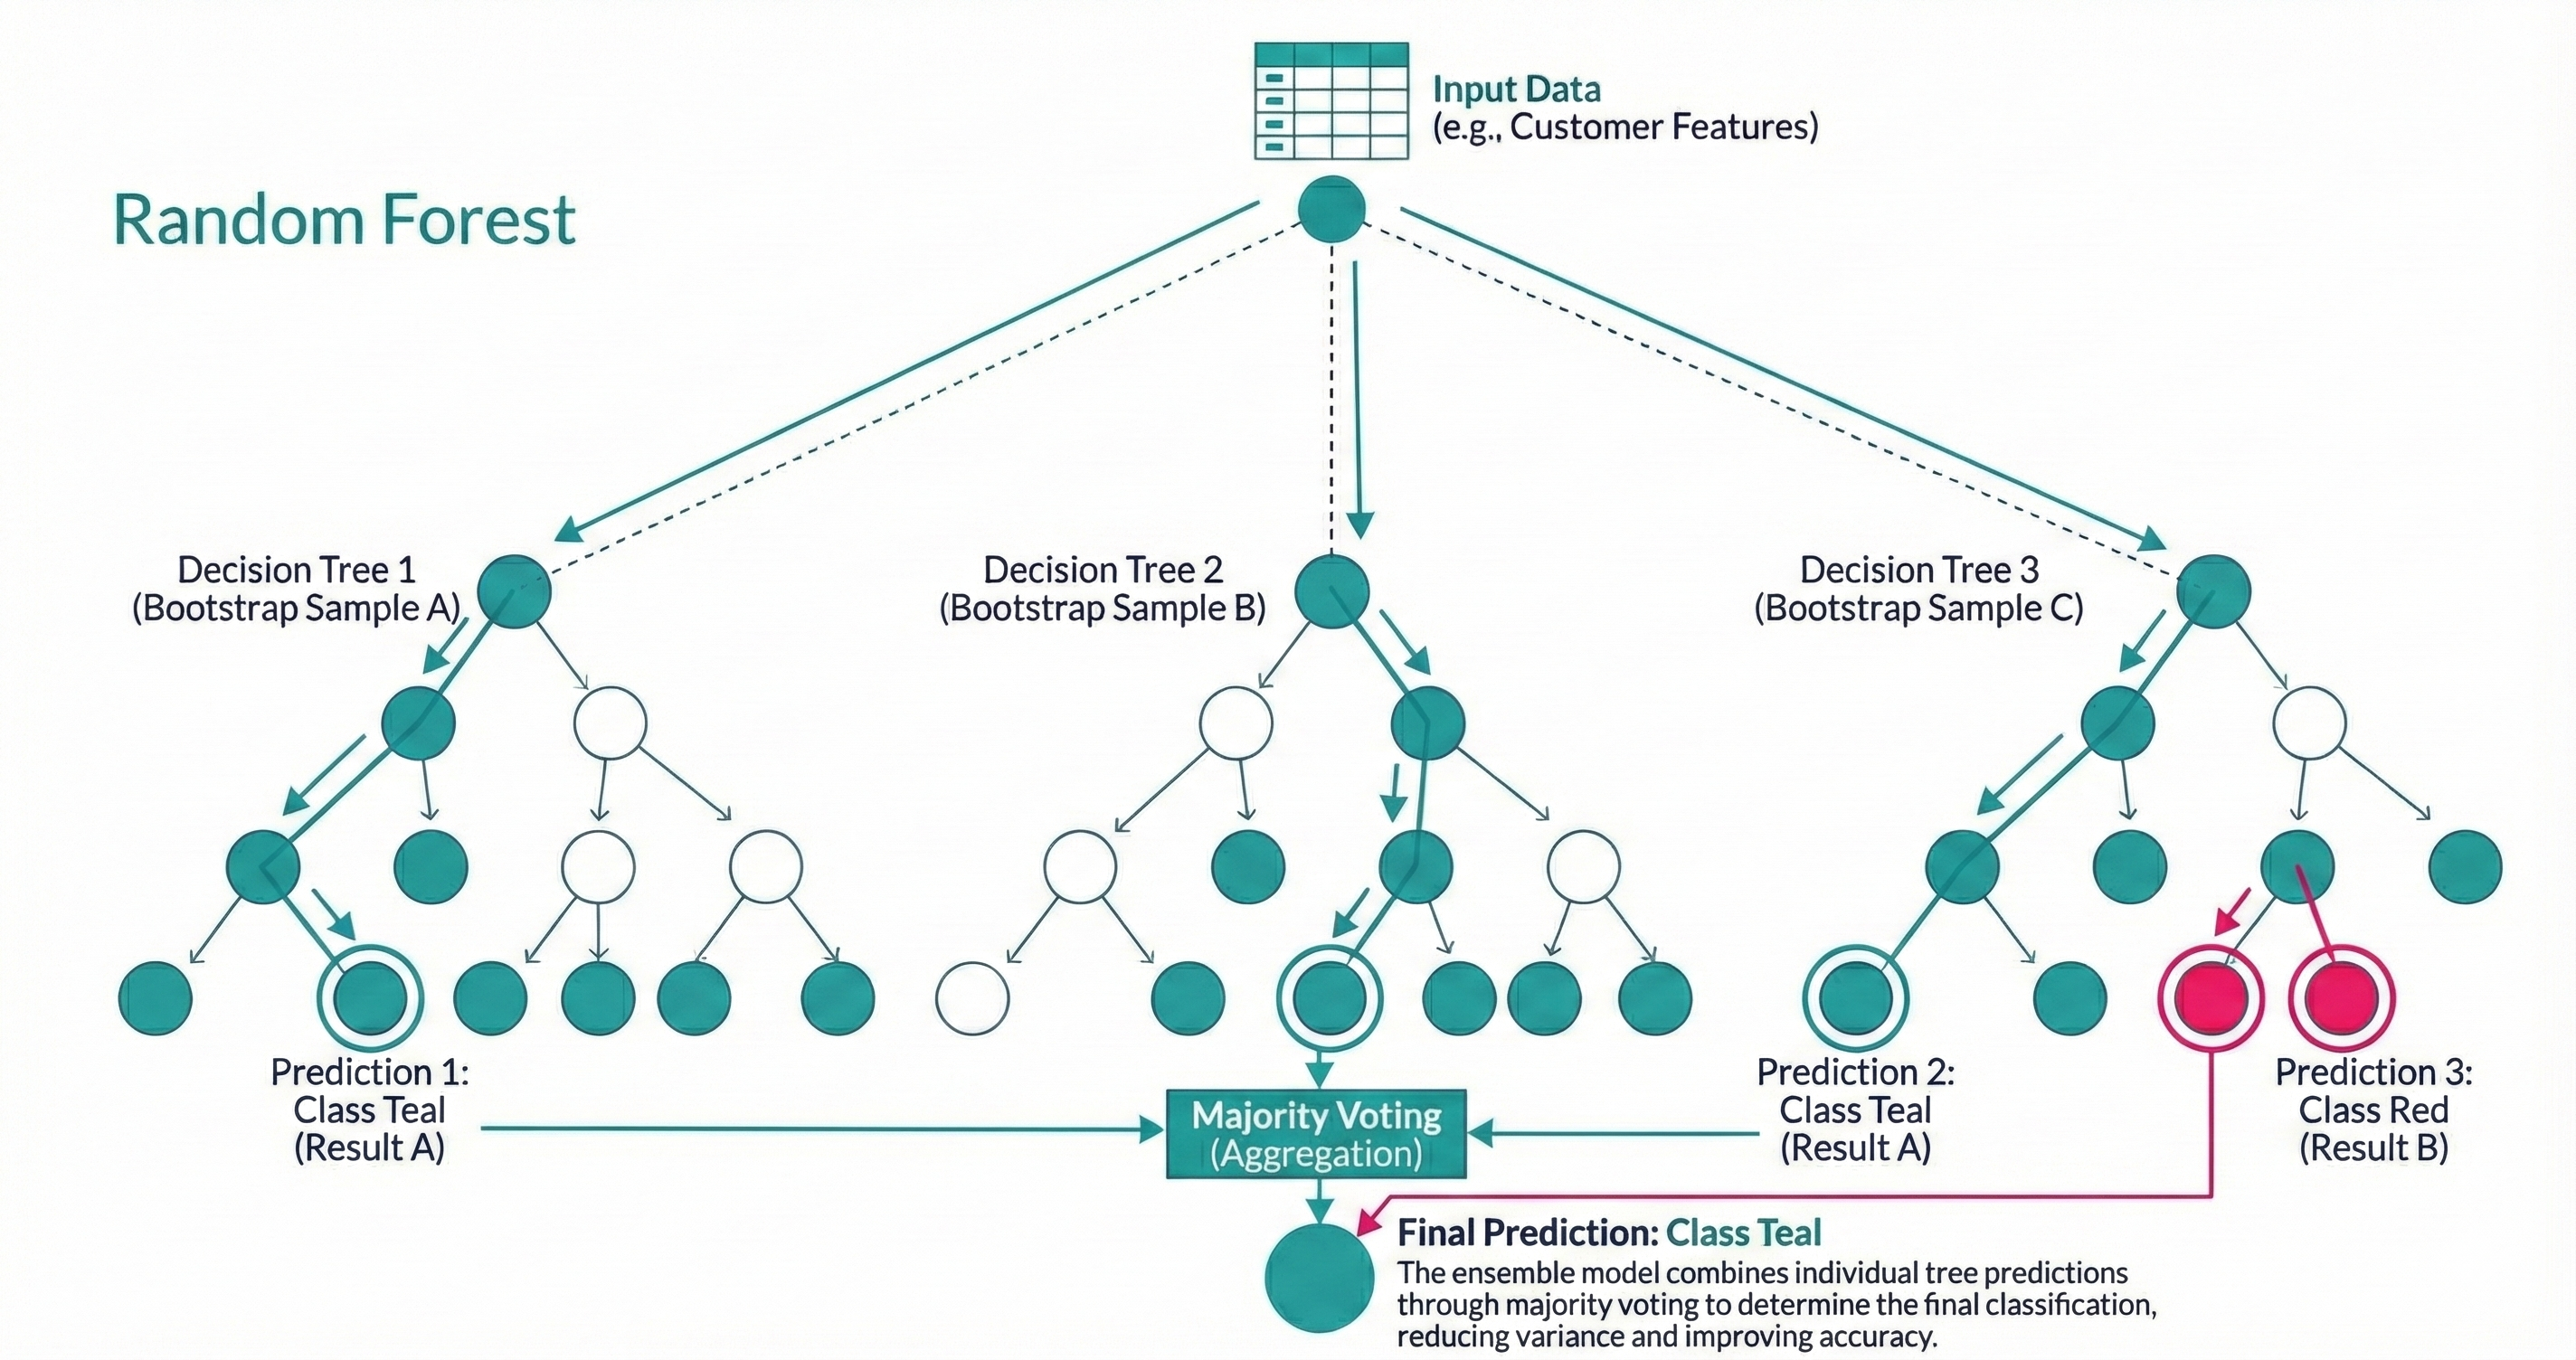
\includegraphics[width=0.9\linewidth]{Random_Forest.jpg}
    \caption{Diagram illustrating the Random Forest algorithm and majority voting process.}
    \label{fig:randomforest_diagram}
\end{figure}

\subsection*{Effect on Bias and Variance}

\begin{itemize}
    \item Each tree is a high-variance, low-bias model.
    \item Averaging many trees reduces variance while keeping bias roughly the same.
    \item This usually improves generalization significantly.
\end{itemize}

\subsection*{Important Hyperparameters}

\begin{itemize}
    \item \texttt{n\_estimators}: 
          Controls the \textbf{number of trees} in the forest.  
          This affects the \emph{ensemble level}: more trees usually reduce variance
          and improve stability.

    \item \texttt{max\_depth}:  
          Limits the \textbf{maximum depth of each individual tree}.  
          Acts at the \emph{tree level}.  
          Smaller depth → simpler trees → less overfitting.

    \item \texttt{max\_features}:  
          Controls how many features are considered when searching for the best split
          \emph{at each node}.  
          Acts at the \emph{split level}.  
          Adding randomness here reduces correlation between trees.

    \item \texttt{min\_samples\_leaf}:  
          Sets the minimum number of samples required to form a leaf.  
          Acts at the \emph{leaf level}.  
          Larger values force leaves to contain more data → smoother predictions.
\end{itemize}


\subsection*{Python Example: Random Forest Regression}

\begin{mlcode}
\begin{lstlisting}[style=pystyle, language=Python, title=Random Forest Regression Example]
from sklearn.ensemble import RandomForestRegressor
from sklearn.datasets import fetch_california_housing
from sklearn.model_selection import train_test_split
from sklearn.metrics import mean_squared_error

# Load dataset
data = fetch_california_housing()
X, y = data.data, data.target

# Split data
X_train, X_test, y_train, y_test = train_test_split(
    X, y, test_size=0.2, random_state=42
)

# Train model
forest = RandomForestRegressor(
    n_estimators=200,
    max_depth=None,
    random_state=42
)
forest.fit(X_train, y_train)

#forest = RandomForestRegressor(
#    n_estimators=300,          # number of trees
#    max_depth=12,              # maximum depth of each tree
#    max_features="sqrt",       # number of features tested at each split
#    min_samples_leaf=3,        # minimum samples per leaf
#    min_samples_split=4,       # minimum samples required to #split a node
#    random_state=42            # reproducibility
#)

# Predict
y_pred = forest.predict(X_test)

# Evaluate
mse = mean_squared_error(y_test, y_pred)
print("Random Forest MSE:", mse)
\end{lstlisting}
\end{mlcode}


\begin{mlcode}
\begin{lstlisting}[style=pystyle, language=Python, 
title=Random Forest Regression on Synthetic $\sin(x)$ Data (with Plot)]

import numpy as np
import matplotlib.pyplot as plt
from sklearn.model_selection import train_test_split
from sklearn.ensemble import RandomForestRegressor
from sklearn.metrics import mean_squared_error

# ---------------------------------------------------------
# 1. Create synthetic data for y = sin(x) + noise
# ---------------------------------------------------------
np.random.seed(0)

n_samples = 200
X = np.linspace(0, 2*np.pi, n_samples).reshape(-1, 1)
y_true_function = np.sin(X[:, 0])
noise = 0.1 * np.random.randn(n_samples)
y = y_true_function + noise

# ---------------------------------------------------------
# 2. Train-test split
# ---------------------------------------------------------
X_train, X_test, y_train, y_test = train_test_split(
    X, y, test_size=0.2, random_state=42
)

# ---------------------------------------------------------
# 3. Random Forest model
# ---------------------------------------------------------
forest = RandomForestRegressor(
    n_estimators=200,
    max_depth=8,
    random_state=42
)

# ---------------------------------------------------------
# 4. Train the model
# ---------------------------------------------------------
forest.fit(X_train, y_train)

# ---------------------------------------------------------
# 5. Predict on test set
# ---------------------------------------------------------
y_pred = forest.predict(X_test)
mse = mean_squared_error(y_test, y_pred)
print("Test MSE (Random Forest on sin(x)):", mse)

# ---------------------------------------------------------
# 6. Plot: true function, noisy data, and model predictions
# ---------------------------------------------------------
# Sort for nice plotting
sort_idx = np.argsort(X_test[:, 0])
X_test_sorted = X_test[sort_idx]
y_test_sorted = y_test[sort_idx]
y_pred_sorted = y_pred[sort_idx]

# High-resolution grid for smooth model curve
X_grid = np.linspace(0, 2*np.pi, 1000).reshape(-1, 1)
y_grid_pred = forest.predict(X_grid)

plt.figure(figsize=(10, 5))

# True function (smooth)
plt.plot(X[:, 0], y_true_function, label="True sin(x)", color="black", linewidth=2)

# Noisy training data
plt.scatter(X_train[:, 0], y_train, label="Noisy training data", alpha=0.5)

# Random Forest smooth prediction
plt.plot(X_grid[:, 0], y_grid_pred, label="Random Forest prediction", color="red", linewidth=2)

plt.legend()
plt.title("Random Forest Regression on Noisy $\sin(x)$ Data")
plt.xlabel("x")
plt.ylabel("y")
plt.grid(True)
plt.show()

# ---------------------------------------------------------
# 7. Print a small table: true vs predicted
# ---------------------------------------------------------
print("\nFirst 10 test points: true vs predicted")
for x_val, y_t, y_p in zip(X_test_sorted[:10, 0],
                           y_test_sorted[:10],
                           y_pred_sorted[:10]):
    print(f"x = {x_val:.2f},  y_true = {y_t:.3f},  y_pred = {y_p:.3f}")
\end{lstlisting}
\end{mlcode}

% ===========================================================
\section{Gradient Boosting}

Random forests build trees in \emph{parallel}.  
Gradient boosting builds trees \emph{sequentially}: each new tree corrects the errors
of the previous model.



\subsection*{Intuition}

We start with a simple model $F_0(x)$ (for example a constant).  
At each step $m = 1, 2, \dots, M$ we add a new tree $h_m(x)$:

\[
F_m(x) = F_{m-1}(x) + \nu \, h_m(x),
\]

where $\nu$ is the learning rate.

\begin{figure}[htbp]
    \centering
    % Adjust the width fraction (e.g., 0.9) to suit your page layout.
    % \linewidth makes it as wide as the current text block.
    \includegraphics[width=0.9\linewidth]{gradient.jpg}
    \caption{Diagram illustrating the Gradient Boosting. }
    \label{fig:gradient_boosting_diagram}
\end{figure}

What does $h_m(x)$ learn?  
It is trained to fit the \textbf{residuals} of the previous model:

\[
r_i^{(m)} = y_i - F_{m-1}(x_i).
\]

So each tree focuses on what the current model is doing badly.

\begin{mlidea}
Random forest: many independent trees averaged.  
Gradient boosting: a sequence of trees, each correcting the previous ones.
\end{mlidea}

\subsection*{Optimization View}

More generally, gradient boosting fits trees to the \emph{negative gradient} of the loss
function with respect to the current predictions.  
This is why it is called \textbf{gradient} boosting.

\medskip

To see this mathematically, suppose our model at iteration $m$ is $F_{m-1}(x)$,
and we want to minimize the empirical risk
\[
R(F) = \frac{1}{n} \sum_{i=1}^n L\bigl(y_i, F(x_i)\bigr).
\]

The gradient of the loss with respect to the model’s prediction at point $x_i$ is:
\[
g_i^{(m)} = 
\left.\frac{\partial L(y_i, F(x_i))}{\partial F(x_i)}\right|_{F = F_{m-1}}.
\]

Gradient boosting uses the \emph{negative gradient} as a pseudo-target:
\[
r_i^{(m)} = -g_i^{(m)}.
\]

\begin{mlnote}
The negative gradient $r_i^{(m)}$ gives the direction in which the loss decreases the fastest.
For squared loss,
\[
L(y_i, F) = (y_i - F)^2,
\quad\Longrightarrow\quad
r_i^{(m)} = y_i - F_{m-1}(x_i),
\]
so the negative gradient is exactly the \emph{residual}.
\end{mlnote}

\medskip

The new tree $h_m(x)$ is trained to approximate these pseudo-targets:
\[
h_m(x) \approx r^{(m)}.
\]

The model is then updated by taking a small step in that direction:
\[
F_m(x) = F_{m-1}(x) + \nu\, h_m(x),
\]
where $0 < \nu \le 1$ is the learning rate.

\begin{mlidea}
Gradient boosting is gradient descent in \emph{function space}:  
each tree $h_m$ points in the direction that most reduces the loss,  
and the learning rate $\nu$ controls how big that step is.
\end{mlidea}


\subsection*{Hyperparameters}

\begin{itemize}
    \item \texttt{n\_estimators}: number of boosting iterations (trees).
    \item \texttt{learning\_rate} $\nu$: step size; smaller values need more trees.
    \item \texttt{max\_depth}: depth of each individual tree (usually small, e.g.\ 3--5).
\end{itemize}

\subsection*{Python Example: Gradient Boosting Regression}

\begin{mlcode}
\begin{lstlisting}[style=pystyle, language=Python, title=Gradient Boosting Regression]
from sklearn.ensemble import GradientBoostingRegressor
from sklearn.datasets import fetch_california_housing
from sklearn.model_selection import train_test_split
from sklearn.metrics import mean_squared_error

data = fetch_california_housing()
X, y = data.data, data.target

X_train, X_test, y_train, y_test = train_test_split(
    X, y, test_size=0.2, random_state=42
)

gbr = GradientBoostingRegressor(
    n_estimators=300,
    learning_rate=0.05,
    max_depth=3
)
gbr.fit(X_train, y_train)

y_pred = gbr.predict(X_test)
print("GBR MSE:", mean_squared_error(y_test, y_pred))
\end{lstlisting}
\end{mlcode}

\begin{mlcode}
\begin{lstlisting}[style=pystyle, language=Python,
title=Gradient Boosting Regression on Synthetic $\sin(x)$ Data (with Plot)]

import numpy as np
import matplotlib.pyplot as plt
from sklearn.model_selection import train_test_split
from sklearn.ensemble import GradientBoostingRegressor
from sklearn.metrics import mean_squared_error

# ---------------------------------------------------------
# 1. Create synthetic data for y = sin(x) + noise
#    (same setup as for the Random Forest example)
# ---------------------------------------------------------
np.random.seed(0)

n_samples = 200
X = np.linspace(0, 2*np.pi, n_samples).reshape(-1, 1)
y_true_function = np.sin(X[:, 0])
noise = 0.1 * np.random.randn(n_samples)
y = y_true_function + noise

# ---------------------------------------------------------
# 2. Train-test split
# ---------------------------------------------------------
X_train, X_test, y_train, y_test = train_test_split(
    X, y, test_size=0.2, random_state=42
)

# ---------------------------------------------------------
# 3. Gradient Boosting model
# ---------------------------------------------------------
# n_estimators  : number of boosting stages (trees)
# learning_rate : step size for each tree's contribution
# max_depth     : depth of individual regression trees
# random_state  : reproducibility

gboost = GradientBoostingRegressor(
    n_estimators=300,
    learning_rate=0.05,
    max_depth=3,
    random_state=42
)

# ---------------------------------------------------------
# 4. Train the model
# ---------------------------------------------------------
gboost.fit(X_train, y_train)

# ---------------------------------------------------------
# 5. Predict on test set and compute MSE
# ---------------------------------------------------------
y_pred = gboost.predict(X_test)
mse = mean_squared_error(y_test, y_pred)
print("Test MSE (Gradient Boosting on sin(x)):", mse)

# ---------------------------------------------------------
# 6. Plot: true function, noisy data, and GB prediction
# ---------------------------------------------------------
# Sort for nice plotting
sort_idx = np.argsort(X_test[:, 0])
X_test_sorted = X_test[sort_idx]
y_test_sorted = y_test[sort_idx]
y_pred_sorted = y_pred[sort_idx]

# High-resolution grid for smooth model curve
X_grid = np.linspace(0, 2*np.pi, 1000).reshape(-1, 1)
y_grid_pred = gboost.predict(X_grid)

plt.figure(figsize=(10, 5))

# True function (smooth)
plt.plot(X[:, 0], y_true_function, label="True sin(x)", color="black", linewidth=2)

# Noisy training data
plt.scatter(X_train[:, 0], y_train, label="Noisy training data", alpha=0.5)

# Gradient Boosting prediction
plt.plot(X_grid[:, 0], y_grid_pred, label="Gradient Boosting prediction",
         color="green", linewidth=2)

plt.legend()
plt.title("Gradient Boosting Regression on Noisy $\sin(x)$ Data")
plt.xlabel("x")
plt.ylabel("y")
plt.grid(True)
plt.show()

# ---------------------------------------------------------
# 7. Print a small table: true vs predicted
# ---------------------------------------------------------
print("\nFirst 10 test points: true vs predicted (Gradient Boosting)")
for x_val, y_t, y_p in zip(X_test_sorted[:10, 0],
                           y_test_sorted[:10],
                           y_pred_sorted[:10]):
    print(f"x = {x_val:.2f},  y_true = {y_t:.3f},  y_pred = {y_p:.3f}")
\end{lstlisting}
\end{mlcode}


% ===========================================================
\section{XGBoost: Extreme Gradient Boosting}

Now we can finally answer: \textbf{What is XGBoost?}

XGBoost is a specific, highly optimized implementation of gradient boosting for decision trees.
It uses the same basic idea (add trees sequentially to correct errors), but introduces:

\begin{itemize}
    \item strong regularization of trees,
    \item second-order (Hessian) information,
    \item efficient handling of sparse inputs,
    \item parallelization and system optimizations.
\end{itemize}

Because of these improvements, XGBoost tends to be:
\begin{itemize}
    \item faster to train,
    \item more accurate,
    \item better at controlling overfitting,
\end{itemize}
than a naive gradient boosting implementation.

\subsection*{Objective Function}

The model at iteration $t$ is:

\[
\hat{y}_i^{(t)} = \sum_{k=1}^{t} f_k(x_i),
\]
where each $f_k$ is a decision tree.

XGBoost minimizes the regularized objective:

\[
\mathcal{L}^{(t)} =
\sum_{i=1}^n L\big(y_i, \hat{y}_i^{(t-1)} + f_t(x_i)\big)
+ \Omega(f_t),
\]

with regularization term:

\[
\Omega(f_t) = \gamma T + \frac{1}{2}\lambda \sum_{j=1}^{T} w_j^2,
\]

where:
\begin{itemize}
    \item $T$ = number of leaves in the tree,
    \item $w_j$ = weight (value) assigned to leaf $j$,
    \item $\gamma$ and $\lambda$ are regularization hyperparameters.
\end{itemize}

This penalizes both the \emph{size} of the tree (number of leaves) and the
\emph{magnitude} of leaf weights, which helps prevent overfitting.

\subsection*{Second-Order Approximation}

To efficiently choose splits and leaf values, XGBoost uses a second-order
Taylor expansion of the loss around the current predictions:

\[
L(y_i, \hat{y}_i^{(t-1)} + f_t(x_i))
\approx
L(y_i, \hat{y}_i^{(t-1)})
+ g_i f_t(x_i)
+ \frac{1}{2} h_i f_t(x_i)^2,
\]

where:
\begin{itemize}
    \item $g_i = \partial_{\hat{y}} L(y_i, \hat{y}_i^{(t-1)})$ (gradient),
    \item $h_i = \partial^2_{\hat{y}} L(y_i, \hat{y}_i^{(t-1)})$ (Hessian).
\end{itemize}

This second-order information makes tree construction more accurate and efficient.

\subsection*{Key Hyperparameters (What you tune in practice)}

\begin{itemize}
    \item \texttt{n\_estimators}: number of boosting rounds (trees).
    \item \texttt{learning\_rate}: shrinkage factor for each tree contribution.
    \item \texttt{max\_depth}: maximum depth of each tree.
    \item \texttt{subsample}: fraction of training data used per tree.
    \item \texttt{colsample\_bytree}: fraction of features used per tree.
    \item \texttt{reg\_lambda}, \texttt{reg\_alpha}: L2 and L1 regularization on leaf weights.
\end{itemize}

\subsection*{XGBoost Classification Example}

\begin{mlcode}
\begin{lstlisting}[style=pystyle, language=Python, title=XGBoost Classifier]
from xgboost import XGBClassifier
from sklearn.datasets import load_breast_cancer
from sklearn.model_selection import train_test_split
from sklearn.metrics import accuracy_score

data = load_breast_cancer()
X, y = data.data, data.target

X_train, X_test, y_train, y_test = train_test_split(
    X, y, test_size=0.2, random_state=42
)

model = XGBClassifier(
    n_estimators=300,
    learning_rate=0.05,
    max_depth=4,
    subsample=0.8,
    colsample_bytree=0.8,
    eval_metric="logloss"
)

model.fit(X_train, y_train)
y_pred = model.predict(X_test)

print("XGBoost Accuracy:", accuracy_score(y_test, y_pred))
\end{lstlisting}
\end{mlcode}

\subsection*{XGBoost Regression Example}

\begin{mlcode}
\begin{lstlisting}[style=pystyle, language=Python, title=XGBoost Regressor]
from xgboost import XGBRegressor
from sklearn.datasets import fetch_california_housing
from sklearn.model_selection import train_test_split
from sklearn.metrics import mean_squared_error

data = fetch_california_housing()
X, y = data.data, data.target

X_train, X_test, y_train, y_test = train_test_split(
    X, y, test_size=0.2, random_state=42
)

model = XGBRegressor(
    n_estimators=400,
    learning_rate=0.05,
    max_depth=5,
    subsample=0.8,
    colsample_bytree=0.8,
    eval_metric="rmse"
)

model.fit(X_train, y_train)
y_pred = model.predict(X_test)

print("XGBRegressor MSE:", mean_squared_error(y_test, y_pred))
\end{lstlisting}
\end{mlcode}


\begin{mlcode}
\begin{lstlisting}[style=pystyle, language=Python,
title=XGBoost Regression on Synthetic $\sin(x)$ Data (with Plot)]

import numpy as np
import matplotlib.pyplot as plt
from sklearn.model_selection import train_test_split
from sklearn.metrics import mean_squared_error

from xgboost import XGBRegressor   # pip install xgboost

# ---------------------------------------------------------
# 1. Create synthetic data for y = sin(x) + noise
#    (same setup as RF and Gradient Boosting examples)
# ---------------------------------------------------------
np.random.seed(0)

n_samples = 200
X = np.linspace(0, 2*np.pi, n_samples).reshape(-1, 1)
y_true_function = np.sin(X[:, 0])
noise = 0.1 * np.random.randn(n_samples)
y = y_true_function + noise

# ---------------------------------------------------------
# 2. Train-test split
# ---------------------------------------------------------
X_train, X_test, y_train, y_test = train_test_split(
    X, y, test_size=0.2, random_state=42
)

# ---------------------------------------------------------
# 3. XGBoost model
# ---------------------------------------------------------
# n_estimators      : number of boosting trees
# learning_rate     : step size (eta)
# max_depth         : depth of individual trees
# subsample         : fraction of rows used per tree (stochasticity)
# colsample_bytree  : fraction of features used per tree
# reg_lambda        : L2 regularization
# objective         : regression with squared loss

xgb_model = XGBRegressor(
    n_estimators=400,
    learning_rate=0.05,
    max_depth=3,
    subsample=0.9,
    colsample_bytree=0.9,
    reg_lambda=1.0,
    objective="reg:squarederror",
    random_state=42
)

# ---------------------------------------------------------
# 4. Train the model
# ---------------------------------------------------------
xgb_model.fit(X_train, y_train)

# ---------------------------------------------------------
# 5. Predict on test set and compute MSE
# ---------------------------------------------------------
y_pred = xgb_model.predict(X_test)
mse = mean_squared_error(y_test, y_pred)
print("Test MSE (XGBoost on sin(x)):", mse)

# ---------------------------------------------------------
# 6. Plot: true function, noisy data, and XGBoost prediction
# ---------------------------------------------------------
# Sort test data for nicer display
sort_idx = np.argsort(X_test[:, 0])
X_test_sorted = X_test[sort_idx]
y_test_sorted = y_test[sort_idx]
y_pred_sorted = y_pred[sort_idx]

# High-resolution grid for smooth model curve
X_grid = np.linspace(0, 2*np.pi, 1000).reshape(-1, 1)
y_grid_pred = xgb_model.predict(X_grid)

plt.figure(figsize=(10, 5))

# True function
plt.plot(X[:, 0], y_true_function, label="True sin(x)",
         color="black", linewidth=2)

# Noisy training data
plt.scatter(X_train[:, 0], y_train, label="Noisy training data",
            alpha=0.5)

# XGBoost prediction
plt.plot(X_grid[:, 0], y_grid_pred, label="XGBoost prediction",
         color="purple", linewidth=2)

plt.legend()
plt.title("XGBoost Regression on Noisy $\sin(x)$ Data")
plt.xlabel("x")
plt.ylabel("y")
plt.grid(True)
plt.show()

# ---------------------------------------------------------
# 7. Print a small table: true vs predicted
# ---------------------------------------------------------
print("\nFirst 10 test points: true vs predicted (XGBoost)")
for x_val, y_t, y_p in zip(X_test_sorted[:10, 0],
                           y_test_sorted[:10],
                           y_pred_sorted[:10]):
    print(f"x = {x_val:.2f},  y_true = {y_t:.3f},  y_pred = {y_p:.3f}")
\end{lstlisting}
\end{mlcode}

% ===========================================================
\newpage
\section{Summary: Recognizing and Distinguishing the Algorithms}

\begin{mlexample1}
\textbf{How to quickly identify each model}

\begin{itemize}
    \item \textbf{Decision Tree}
    \begin{itemize}
        \item Single tree, flowchart-like structure.
        \item Splits the data based on feature thresholds.
        \item Very interpretable but can overfit easily.
    \end{itemize}

    \item \textbf{Random Forest}
    \begin{itemize}
        \item Many trees trained on bootstrap samples and random subsets of features.
        \item Predictions are averaged (regression) or voted (classification).
        \item Reduces variance and is robust; default strong baseline.
    \end{itemize}

    \item \textbf{Gradient Boosting}
    \begin{itemize}
        \item Trees are added one after another.
        \item Each new tree focuses on residuals / gradients of the previous model.
        \item Can fit complex patterns with relatively shallow trees.
    \end{itemize}

    \item \textbf{XGBoost / XGBRegressor}
    \begin{itemize}
        \item A particular implementation of tree-based gradient boosting.
        \item Uses regularization, second-order gradients, and many optimizations.
        \item Often achieves state-of-the-art performance on tabular datasets.
    \end{itemize}
\end{itemize}

\textbf{Rule of thumb:}
\begin{itemize}
    \item Need interpretability and a quick idea? Try a single \emph{decision tree}.
    \item Need a strong, robust model with little tuning? Use a \emph{random forest}.
    \item Need maximum performance and are willing to tune hyperparameters?  
          Use \emph{gradient boosting} or \emph{XGBoost}.
\end{itemize}
\end{mlexample1}

% =======================


% =======================
\chapter{Neural Networks \& Deep Learning}

Neural networks are among the most powerful and widely used models in modern
machine learning. They are capable of learning highly nonlinear relationships,
complex patterns in images, speech, text, and even reinforcement-learning tasks.

This chapter presents the essential ideas behind neural networks and deep
learning in a clear, intuitive, and mathematically grounded way.

\section*{What Makes Neural Networks Special?}

Neural networks do not rely on manually–designed features.
Instead, they learn representations directly from data.

\begin{mlidea}
Neural networks learn \emph{hierarchies of features}:  
simple patterns at shallow layers, more complex patterns at deeper layers.
\end{mlidea}

They are versatile enough to solve:
\begin{itemize}
    \item regression problems,
    \item classification problems,
    \item image analysis (CNNs),
    \item sequential modelling (RNNs, LSTMs, Transformers),
    \item reinforcement learning,
    \item generative modelling.
\end{itemize}

In this chapter we focus on the foundations needed to understand all these models.


% ============================================================
\section{The Perceptron: The Simplest Neural Unit}

The basic building block of a neural network is the \textbf{neuron} (or node).
The simplest neuron is the classical \textbf{perceptron}.

\subsection*{Mathematical Form}

Given an input vector $x \in \mathbb{R}^d$:

\[
z = w^\top x + b
\]

and an activation:

\[
\hat{y} = \sigma(z)
\]

where:
\begin{itemize}
    \item $w$ = weights,
    \item $b$ = bias,
    \item $\sigma(\cdot)$ = activation function.
\end{itemize}

\subsection*{Activation Functions}

\[ \sigma(z) \text{ introduces nonlinearity.} \]

Common functions:
\begin{itemize}
    \item \textbf{Sigmoid:} 
    \[
    \sigma(z) = \frac{1}{1 + e^{-z}}
    \]
    \item \textbf{ReLU:}
    \[
    \sigma(z) = \max(0, z)
    \]
    \item \textbf{Tanh:}
    \[
    \sigma(z) = \tanh(z)
    \]
\end{itemize}

\begin{mlidea}
If we remove activation functions, a neural network collapses into a linear regression model.
Nonlinear activations give neural networks their expressive power.
\end{mlidea}


% ============================================================
\section{Multi–Layer Perceptron (MLP)}

A \textbf{Multi–Layer Perceptron} is a sequence of layers:

\[
\text{input} \to \text{hidden layers} \to \text{output}.
\]

Each layer transforms the previous layer via linear combination + activation.

\subsection*{Structure}

\[
\begin{aligned}
h^{(1)} &= \sigma\left(W^{(1)} x + b^{(1)}\right), \\
h^{(2)} &= \sigma\left(W^{(2)} h^{(1)} + b^{(2)}\right), \\
\vdots  \\
\hat{y} &= W^{(L)} h^{(L-1)} + b^{(L)}.
\end{aligned}
\]

\begin{center}
\texttt{
Input → Layer 1 → Layer 2 → ... → Output  
}
\end{center}

Each layer increases the model’s ability to capture patterns.

\begin{mlnote}
A neural network with one hidden layer and enough neurons can approximate \emph{any continuous function}.  
This is the \textbf{Universal Approximation Theorem}.
\end{mlnote}

% ============================================================
\section{Forward Pass and Loss Function}

During training, the network performs:

\begin{enumerate}
    \item \textbf{Forward pass:} compute predictions $\hat{y}$.
    \item \textbf{Compute loss:} measure how wrong the predictions are.
    \item \textbf{Backward pass:} compute gradients of the loss with respect to each parameter.
    \item \textbf{Parameter update:} adjust weights to reduce the loss.
\end{enumerate}

For regression, the loss is MSE:

\[
L = \frac{1}{n}\sum (y_i - \hat{y}_i)^2.
\]

For classification, the loss is cross–entropy:

\[
L = -\sum y_i \log(\hat{p}_i).
\]


% ============================================================
\section{Backpropagation: How Neural Networks Learn}

Backpropagation is the algorithm that computes all gradients efficiently.

\subsection*{Chain Rule}

Backprop uses the chain rule repeatedly:

\[
\frac{\partial L}{\partial W^{(l)}}
=
\frac{\partial L}{\partial h^{(l)}}
\cdot
\frac{\partial h^{(l)}}{\partial z^{(l)}}
\cdot
\frac{\partial z^{(l)}}{\partial W^{(l)}}.
\]

This allows gradients to flow from the output backward.

\begin{mlidea}
Backpropagation = computationally efficient application of the chain rule.
\end{mlidea}


% ============================================================
\section{Training with Gradient Descent}

Once we have gradients, we update each parameter:

\[
W \leftarrow W - \eta \, \frac{\partial L}{\partial W},
\]

where $\eta$ is the learning rate.

Variants include:
\begin{itemize}
    \item SGD (stochastic gradient descent)
    \item Adam
    \item RMSProp
    \item Momentum methods
\end{itemize}

\begin{mlnote}
The learning rate is one of the most important hyperparameters.  
Too large → divergence.  
Too small → very slow learning.
\end{mlnote}


% ============================================================
\section{Why Deep Networks Work}

Deep networks work because each layer extracts more abstract information:

\begin{itemize}
    \item shallow layers learn local, simple patterns,
    \item deeper layers learn more complex concepts.
\end{itemize}

In image classification:
\begin{itemize}
    \item layer 1 learns edges,
    \item layer 2 learns textures,
    \item layer 3 learns object parts,
    \item final layers learn entire objects.
\end{itemize}

Deep learning = \textbf{stacking many layers of representation learning}.


% ============================================================
\section{Overfitting and Regularization in Neural Networks}

Neural networks have many parameters, so overfitting is common.

\subsection*{Regularization techniques}

\begin{itemize}
    \item \textbf{L2 weight decay}
    \item \textbf{Dropout}
    \item \textbf{Early stopping}
    \item \textbf{Batch Normalization}
\end{itemize}

\begin{mlidea}
Dropout randomly disables neurons during training to prevent co-adaptation.  
This forces the network to learn more robust representations.
\end{mlidea}

\newpage
\begin{figure}[h!]
    \centering
    % Adjust the width fraction (e.g., 0.9) to suit your page layout.
    % \linewidth makes it as wide as the current text block.
    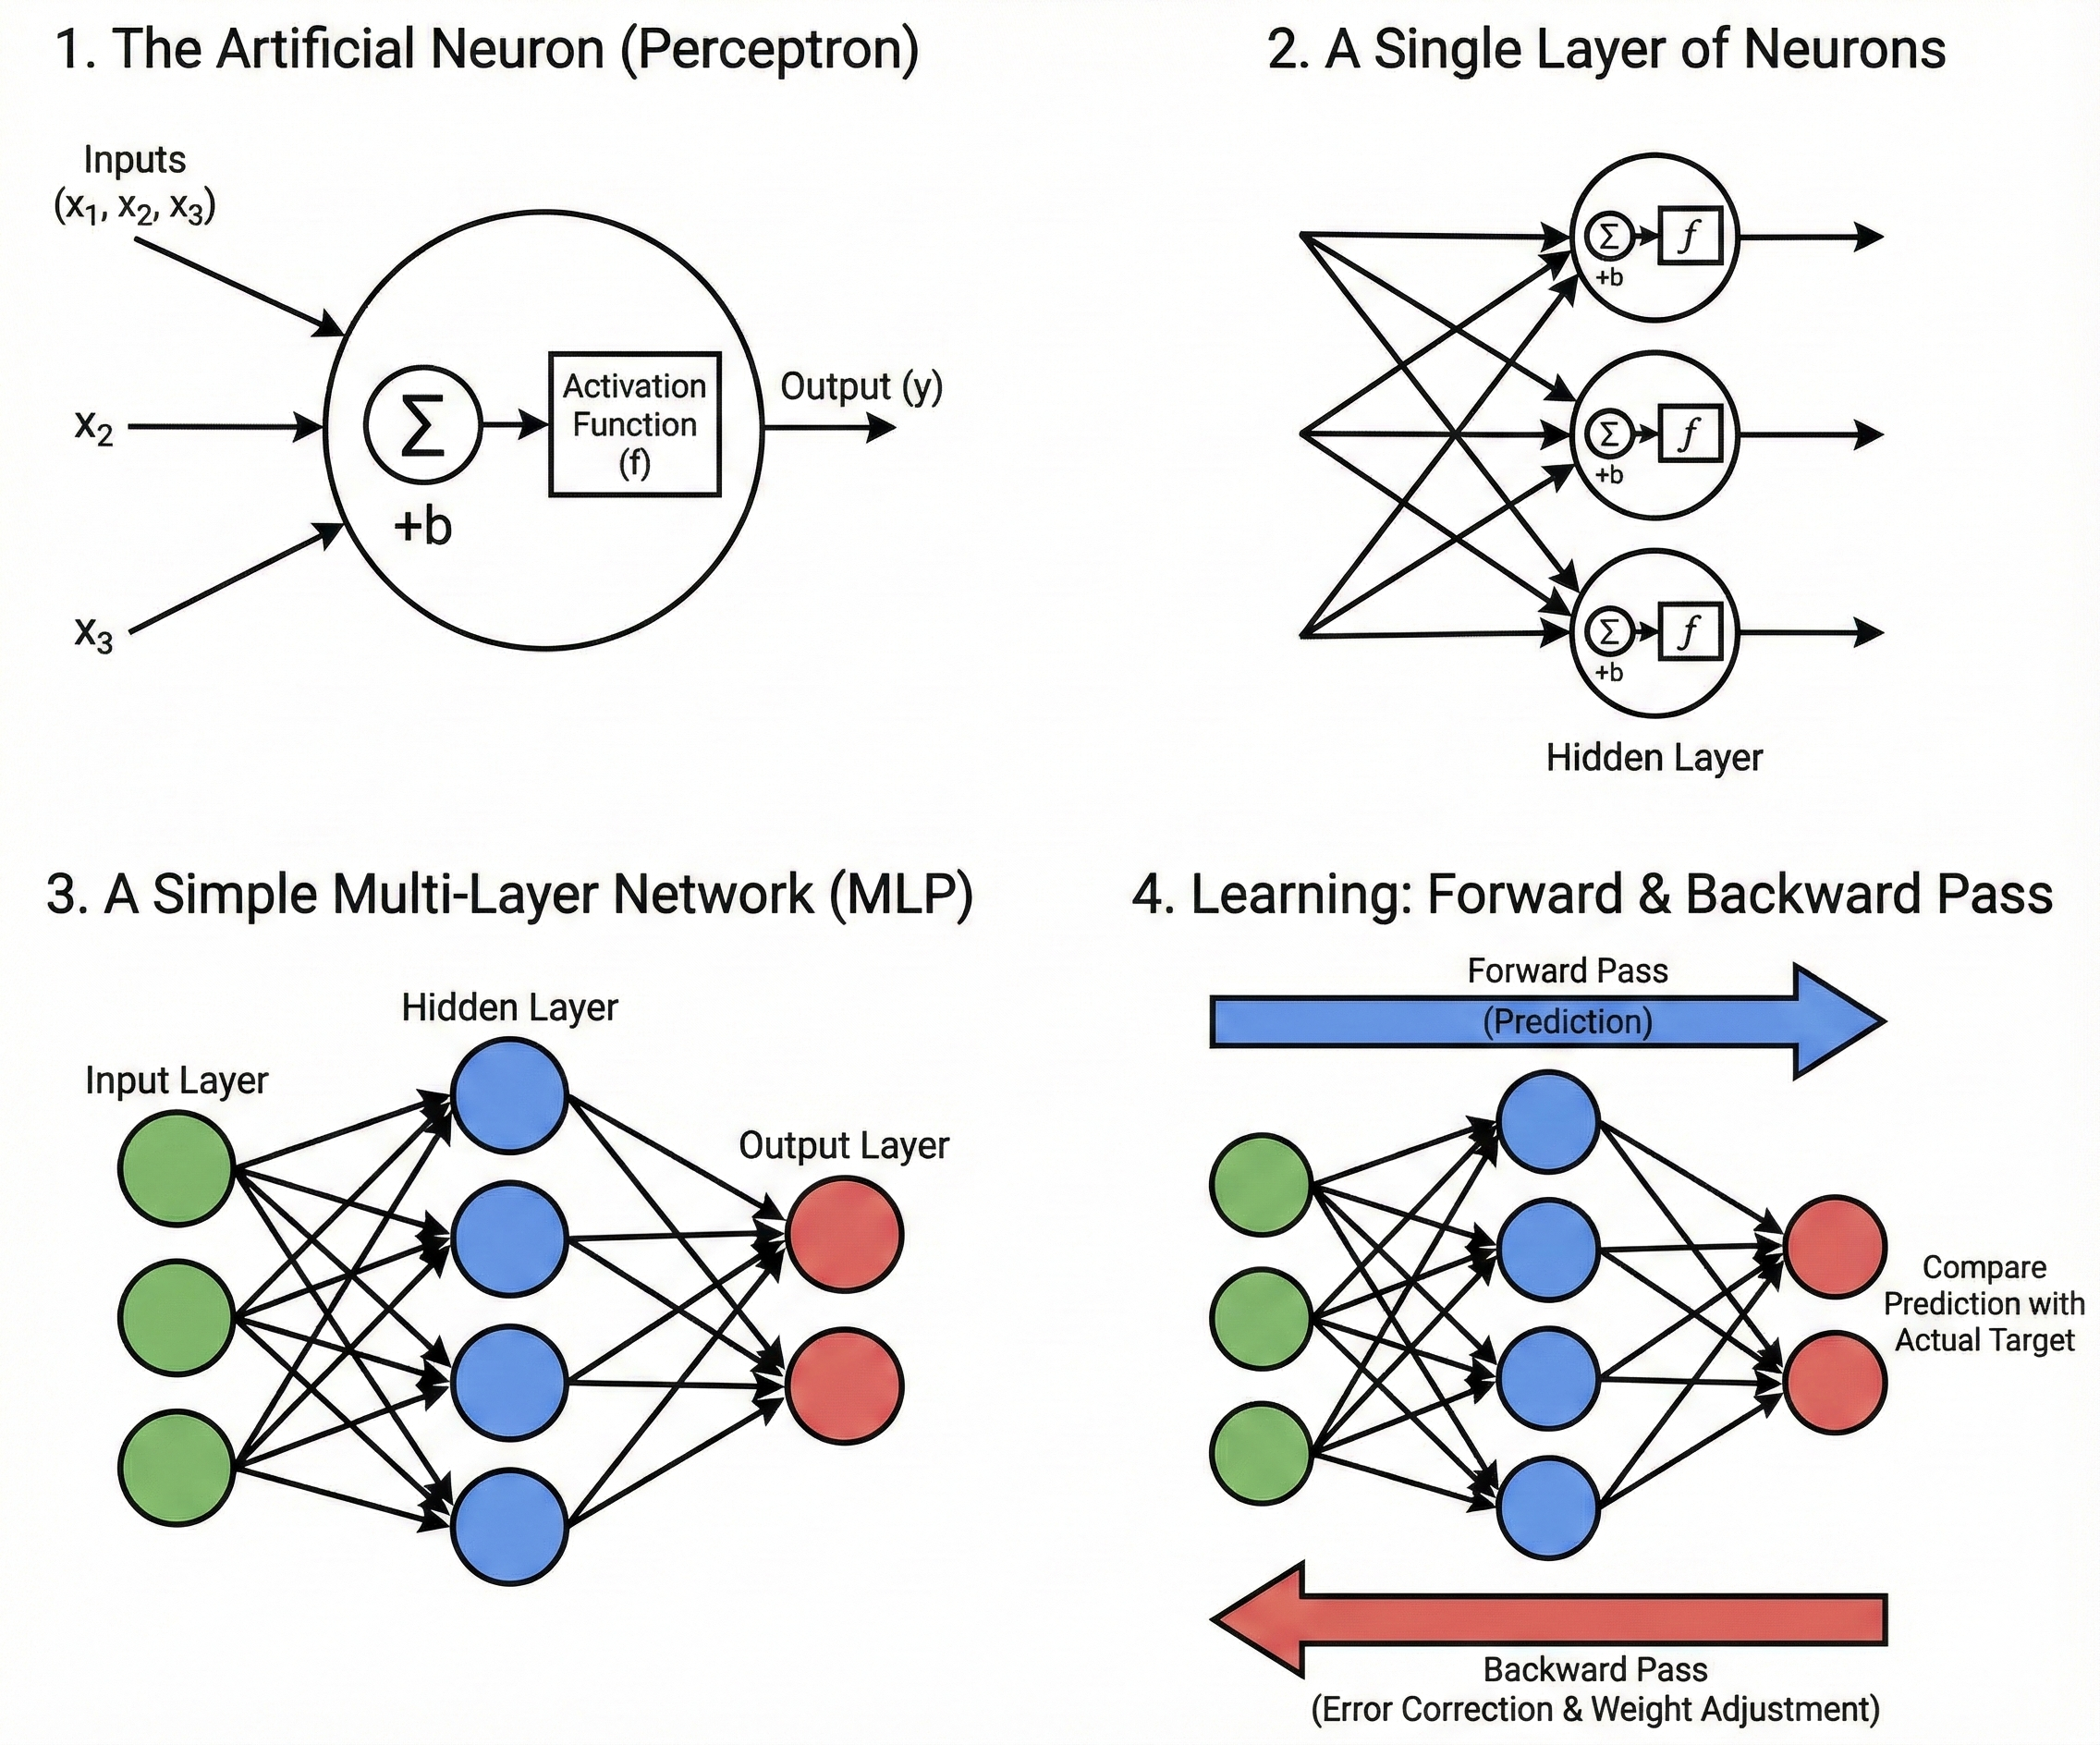
\includegraphics[width=0.99\linewidth]{neuralall.png}
\caption{\textbf{From Neuron to Network: The Anatomy of Deep Learning.} Visualizing the hierarchy of a neural network: individual inputs ($x$) are processed by neurons using weights ($w$) and biases ($b$), then stacked into layers to form a complete Deep Learning architecture.}
    \label{fig:neural_network_diagram}
\end{figure}

% ============================================================
\section{Python Example: Neural Network for Classification (Keras)}

Below is a minimal neural network for binary classification (breast cancer dataset).

\begin{mlcode}
\begin{lstlisting}[style=pystyle, language=Python, title=Neural Network (Keras)]
from sklearn.datasets import load_breast_cancer
from sklearn.model_selection import train_test_split
from sklearn.preprocessing import StandardScaler
from tensorflow.keras.models import Sequential
from tensorflow.keras.layers import Dense
from tensorflow.keras.optimizers import Adam

# Load data
data = load_breast_cancer()
X, y = data.data, data.target

# Scale features
scaler = StandardScaler()
X = scaler.fit_transform(X)

# Train-test split
X_train, X_test, y_train, y_test = train_test_split(
    X, y, test_size=0.2, random_state=42
)

# Build model
model = Sequential([
    Dense(16, activation='relu', input_shape=(X_train.shape[1],)),
    Dense(8, activation='relu'),
    Dense(1, activation='sigmoid')
])

# Compile model
model.compile(
    optimizer=Adam(learning_rate=0.001),
    loss='binary_crossentropy',
    metrics=['accuracy']
)

# Train
model.fit(X_train, y_train, epochs=20, batch_size=16, verbose=1)

# Evaluate
loss, acc = model.evaluate(X_test, y_test)
print("Accuracy:", acc)
\end{lstlisting}
\end{mlcode}



% ============================================================
\section{Summary: Recognizing Neural Networks}

\begin{mlexample1}
\textbf{Neural networks vs other ML models}

\begin{itemize}
    \item \textbf{Decision Tree / Random Forest / XGBoost}  
          interpretability, tabular data, low–dimensional problems.

    \item \textbf{Neural Networks}  
          excel when:
          \begin{itemize}
              \item large datasets,
              \item high-dimensional inputs (images, audio, text),
              \item complex nonlinear patterns,
              \item end-to-end learning is important.
          \end{itemize}

    \item \textbf{Deep Learning}  
          simply means: many layers → hierarchical representations.
\end{itemize}

\textbf{Key strength:} automatic feature learning.  
\textbf{Key challenge:} requires large data, careful tuning, and GPUs for large models.
\end{mlexample1}




% =======================

% =======================
\chapter{Practical ML}






% =======================

\end{document}
